\documentclass[11pt,oneside]{uhthesis}
\usepackage{subfigure}
\usepackage[linesnumbered,lined,titlenumbered,ruled]{algorithm2e}
\usepackage{amsmath}
\usepackage{amssymb}
\usepackage{amsbsy}
\usepackage{mathpazo}
\usepackage{float}
\usepackage{verbatim} 


%\floatstyle{ruled}
%\restylefloat{table}

\renewcommand{\tablename}{Tabla}
%\dontprintsemicolon

\title{Aprendizaje autom\'atico para clasificar entonemas en segmentos del habla en espa\~nol}
\author{Masiel Villalba Carmenate}
\advisor{MSc. Damian Vald\'es Santiago \\ \hspace{2.8cm} Dra.C. Raquel Mar\'ia Garc\'ia River\'on}
\degree{Licenciado en Ciencia de la Computación}
\faculty{Facultad de Matemática y Computación}
\date{Septiembre de 2020}
\logo{Graphics/uhlogo}
\makenomenclature

\renewcommand{\vec}[1]{\boldsymbol{#1}}
\newcommand{\diff}[1]{\ensuremath{\mathrm{d}#1}}

\begin{document}

\frontmatter
\maketitle
\renewcommand{\bibname}{Referencias}
\begin{dedication}
\emph{A mi mam\'a,\\ por ser la mejor compinche de todas. \\}
\emph{\\A mi pap\'a,\\ por estar so\~nando siempre conmigo. \\} 
\emph{\\A mi tutor Damian,\\ por toda su empat\'ia y su inagotable paciencia. \\}
\emph{\\A los Carmenaticos, \\por ser la familia m\'as linda que se me pod\'ia dar. \\}
\emph{\\A los amigos,\\ por tocar la puerta cuando m\'as cerrado est\'a el coraz\'on.}
\end{dedication}
%\emph{A los  Carmenaticos, por apostar por los buenos prop\'ositos.}
%\chapter*{Opini\'on del tutor}
\begin{opinion}
La ling\"u\'istica computacional es una rama multidisciplinaria que procesa grandes cantidades de textos escritos u orales. En particular, el an\'alisis autom\'atico de textos orales es un reto y se ha centrado en la transcripci\'on ortogr\'afica. El estudio computacional de la entonaci\'on es menos tratado y no abundan los trabajos sobre este t\'opico en habla hispana, idioma con particularidades en este aspecto. 


La tesis presentada por Masiel Villalba Carmenate propone un algoritmo basado en aprendizaje autom\'atico para la clasificaci\'on de segmentos de habla del espa\~nol de Cuba en la tipolog\'ia de entonemas para esta variante del espa\~nol propuesta por la enton\'ologa cubana Dra.C. Raquel Mar\'ia Garc\'ia River\'on. Los entonemas son unidades presentes en la cadena hablada que cumplen funciones sintagm\'aticas y pragm\'aticas, y que interact\'uan con otros niveles ling\"u\'isticos (como la gram\'atica) para construir un significado ling\"u\'istico complejo. Esto hace muy complicado su estudio.


Uno de los inconvenientes afrontados durante la investigaci\'on fue la ausencia de un corpus anotado con la tipolog\'ia de entonemas usada. Por ello, uno de los primeros pasos fue la construcci\'on de dicho corpus. Adem\'as, Masiel sistematiz\'o algunos de los modelos computacionales utilizados para el estudio de la entonaci\'on hisp\'anica, ninguno compatible con el de la Dra.C. Garc\'ia River\'on. Como resultado fundamental se entren\'o y valid\'o un modelo de aprendizaje autom\'atico para clasificar segmentos del habla en la tipolog\'ia de entonemas usada.


Durante el desarrollo del trabajo, Masiel tuvo que estudiar la materia referida, que no est\'a incluida en el curr\'iculo de la carrera y trabaj\'o con ling\"uistas y otros especialistas de la computaci\'on, mostrando disciplina, entrega y rigor. Adem\'as, demostr\'o habilidades para el trabajo con la bibliograf\'ia y  creatividad para proponer soluciones a problemas de implementaci\'on, entre otras competencias de programaci\'on en el lenguaje Python y sus diversos frameworks. Es de destacar el esfuerzo realizado en la construcci\'on del corpus, as\'i como la adaptaci\'on creativa de algunas herramientas para realizar el an\'alisis. Masiel se ha superado y ha sorteado inconvenientes personales e investigativos para lograr terminar esta tesis, donde considero cumpli\'o el objetivo propuesto.



Por tanto, considero que a esta tesis de la estudiante Masiel Villalba Carmenate debe otorg\'arsele la m\'axima calificaci\'on (5 puntos, Excelente), y estoy seguro que en el futuro Masiel se desempe\~nar\'a como una excelente profesional de la Ciencia de la Computaci\'on.


\vfill
\begin{flushleft}
\underline{\hspace{140pt}}\hfill \underline{\hspace{140pt}}\\
MSc. Damian Vald\'es Santiago \hfill Dra.C. Raquel Mar\'ia River\'on \hspace*{7pt}
\end{flushleft}
\end{opinion}
\begin{comment}
content...
\end{comment}



\chapter*{Resumen}
La entonolog\'ia es una ciencia relativamente joven, que se ha ido formando de a poco. Estudia la entonaci\'on, pero, para obtener resultados concretos sobre el comportamiento de este rasgo del enunciado hablado, requiere de grandes corpus anotados de acuerdo a los distintos contornos entonativos observados. Esa tarea de anotar es complicada y extenuante, por eso existe un gran inter\'es en el uso de anotadores autom\'aticos. Para el sistema entonativo cubano, no existe ninguna herramienta como esta, por lo cual en este proyecto se ofrece una propuesta de soluci\'on, que relaciona t\'ecnicas de Aprendizaje Autom\'atico, Aumento de Datos y Procesamiento de Se\~nales con Teor\'ia Wavelet.






\chapter*{Abstract}
The entonology is a relatively young science, that has been formed little by little. It studies intonation, but to obtain concrete results on the behavior of this feature of the spoken utterance, it requires large corpus annotated according to the different intonation contours observed. That task of scoring is complicated and strenuous, which is why there is great interest in the use of automated scorers. For the Cuban intonation system, there is no tool like this, for which in this project a solution proposal is offered, which relates Machine Learning techniques, Data Augmentation and Signal Processing with Wavelet Theory.


\tableofcontents
\listoffigures
\listoftables

\mainmatter

%===================================================================================
% Chapter: Introduction
%===================================================================================
\chapter*{Introducción}\label{chapter:introduction}
\addcontentsline{toc}{chapter}{Introducción}
%===================================================================================

\begin{comment}
janet 1980
cantero 1995

el pudor de desnudarse de los habitos de la lengua propia para acomodarse a los de una lengua extranjera tiene en la entonacion su mas fuerte reducto navarro


Importancia de la entonologia
- sintesis de voz (porque hacer falta anotar bastantes curvas para entrenar una inteligencia rtificial que hable como un cubano x ejemplo)


\cite[dificil de anotar a mano, transcripcion automatica]{silverman1992tobi}

\end{comment}


La entonolog\'ia es la rama de la ciencia que estudia la entonaci\'on. Es triste que, a pesar de lo interesante y necesaria, sea tan poco conocida. Se dice que su establecimiento como rama seria es relativamente joven, aunque su germen data del a\~no 1918 con el \emph{Manual de pronunciaci\'on espa\~nola} \cite{navarro1918manual} del fil\'ologo, bibliotecario y ling\"uista espa\~nol Tom\'as Navarro\footnote{M\'as bien considerado eminente fonetista \cite{garcia1996aspectos1}.}, donde dedica un apartado al fen\'omeno de la entonaci\'on. En su trascendente \emph{Manual de entonaci\'on espa\~nola}~(1944) \cite{tomas1974manual} aborda este tema con mayor plenitud.

Como expresa Navarro:

\begin{quote}
``El conocimiento de la entonaci\'on es, pues, de la mayor importancia tanto para la recta inteligencia de lo que se oye como para la expresi\'on justa de lo que se quiere decir. (...) Es, en fin, cosa sabida que, cuando el tono contradice el sentido de las palabras, se atiende m\'as a lo que aqu\'el significa que a lo que estas representan.''
\end{quote}



esto claro, por la rica informaci\'on que se obtiene a partir de la interpretaci\'on del segmento entonativo:
sentimientos, modalidad oracional, tema del enunciado, intencionalidad del hablante, etc. \cite{vidal2014entonacion}. 



Muchos expertos, como la Dra.C. Raquel Mar\'ia Garc\'ia River\'on, prestigiosa enton\'ologa cubana, insisten en su inclusi\'on en los programas de estudio convencionales, en cursos intensivos para los medios de comunicaci\'on, el teatro y la locuci\'on y para el tratamiento de diversos trastornos de habla \cite{pedrosa2009entonacion}. Afortunadamente se han desarrollado varias investigaciones enfocadas a estudiar estas aplicaciones espec\'ificas \cite{riveronlocutores, marrero2007estudio}.


Otra de las aplicaciones importantes de la entonolog\'ia es la construcci\'on de \emph{mapas pros\'odicos}
que se especializan en la descripci\'on del habla regional. Cabe mencionar en este apartado el \emph{Atlas Ling\"uistico de Cuba} \cite{riveron1991atlas} y el desarrollo del proyecto AMPER \cite{roseanoetiquetaje, ruiz2014entonacion}.


En el \'ambito de la \emph{ling\"u\'istica computacional} genera gran inte\'res tanto para la \emph{síntesis} como para el \emph{reconocimiento de voz}. La transformación de un texto a su correspondiente sonoro implica el uso de la entonación correcta y análogamente sucede en la conversión de habla a texto.


Aunque queda mucho por descubrir y convenciones que adoptar, el andamiaje teórico y metodológico de la entonolog\'ia se ha ido construyendo paulatinamente gracias al inter\'es de muchos estudiosos: Antonio Quilis~(1975) \cite{quilis1975unidades}, Janet Pierrehumbert~(1980) \cite{pierrehumbert1980phonology}, Garrido~(1991) \cite{garrido1991modelizacion}, Cantero~(1995) \cite{cantero1995estructura}, pero, inicialmente, este problema golpeaba fuertemente los avances investigativos. Al respecto se\~nala Navarro:

\begin{quote}
``... el mayor obstáculo con que se tropieza en el estudio de esta materia no consiste tanto en la dificultad de medir la altura de los sonidos, como en la falta de normas adecuadas y eficientes para interpretar y ordenar de un modo apto para la relación comparativa histórica y lingüística, el valor de los resultados que con dichas medidas se obtiene.''
\end{quote}


De todas formas, los recursos técnicos para lIevar a cabo la medición de los indicadores acústicos de la entonación es otro factor que influye en el desarrollo de las investigaciones. Existen diversos instrumentos que han sido históricamente utilizados para esta tarea: el \emph{quimógrafo}, el \emph{oscilógrafo} y el \emph{sonógrafo} \cite{garcia1996aspectos2}. Actualmente la herramienta m\'as utilizada es el software \emph{Praat} \cite{goldman2011easyalign} utilizado para el an\'alisis cient\'ifico del habla de manera general: permite visualizar el \emph{espectrograma} del audio, el cocleagrama, los formantes, etc \cite{ruiz2014entonacion}. 


\subsection*{Problema}

La labor de Garc\'ia River\'on en fortalecer la entonolog\'ia como ciencia y elevar el inter\'es por su estudio ha sido meritoria y sobre todo en Cuba \cite{garcia2004entonacion, garcia2005estudio, riveronuniv, riveronguanta, cubadice, nottelecubana, raquel2018interrogativa, riveroncomplejo}.


En su trilog\'ia \emph{Aspectos de la entonaci\'on hisp\'anica} \cite{garcia1996aspectos1, garcia1996aspectos2, garcia1998aspectos} define y asenta el sistema entonativo cubano, tomando como unidad b\'asica de an\'alisis los llamados \emph{entonemas}, que constituyen patrones de comportamiento de la curva melódica. Cada uno denota intenciones y emociones particulares en el enunciado.


Los especialistas detectan los entonemas a oído, pero necesitan corroborar sus impresiones con distintos instrumentos como los anteriormente mencionados. Esto implica mayor exposición a errores y gasto de tiempo, pues ese segundo paso en la detección, que es la comprobación, no es directo, sino que requiere de cálculos manuales. En fin, se comprueba que esta tarea es particularmente compleja \cite{silverman1992tobi}. Aunque se han construido herramientas para solucionar este problema se necesita una adaptada al sistema entonativo cubano.



\subsection*{Hip\'otesis y Objetivo}
El principal objetivo de esta tesis es desarrollar un anotador autom\'atico que, dado un fragmento de la cadena hablada en la variante cubana del espa\~nol, permita clasificarla en cierta tipolog\'ia de entonemas. Los patrones a reconocer son los 18 planteados por Garc\'ia River\'on \cite[c\'ap. III]{garcia1996aspectos1}.


La hip\'otesis plantea que, basado en los rasgos distintivos de la entonaci\'on establecidos por Garc\'ia River\'on, es posible discriminar entre entonemas por medio de t\'ecnicas de aprendizaje supervisado.

\subsubsection*{Objetivos espec\'ificos}

\begin{enumerate}
\item Estudiar el estado del arte del problema.
\item Experimentar formas diferentes de representar los segmentos de voz para la aplicaci\'on de Aprendizaje Autom\'atico.
\item Estudiar los rasgos distintivos de la entonaci\'on y ver c\'omo traducirlos al entorno matem\'atico.
\item Observar los principales rasgos de preprocesamiento para trabajar con los datos.
\item Construir un corpus etiquetado por entonemas.
\item Identificar un conjunto de algoritmos de aprendizaje.
\end{enumerate}


\section*{Propuesta de soluci\'on}
Se propone la soluci\'on al problema con un enfoque de Aprendizaje Autom\'atico. Los audios de entrada se vectorizan de acuerdo a caracter\'isticas extra\'idas de la curva mel\'odica: entrop\'ia, convoluci\'on, pendiente, espectro de Fourier y coeficientes de detalle en la descomposici\'on del cuarto nivel. Estos rasgos fueron elegidos a partir de las observaciones de Garc\'ia River\'on en sus investigaciones. Para este fin, se necesita construir un corpus anotado por entonemas: para hacerlo m\'as extenso se propone aplicar la t\'ecnica de Aumento de Datos.




\section*{Organizaci\'on de la Tesis}
El documento est\'a organizado de la siguiente manera: en el Cap\'itulo 1 se abordan los conceptos b\'asicos relevantes relacionados con el problema y el estado del arte; en el Cap\'itulo 2 se profundizan las caracter\'isticas del sistema entonativo planteado por la enton\'ologa Garc\'ia River\'on y sus contrastes con otro modelo de transcripci\'on~(sistema ToBI); el Cap\'itulo 3 se destina a la fundamentaci\'on te\'orica de la propuesta de soluci\'on del problema. En el \'ultimo cap\'itulo se expone la metodolog\'ia empleada y los resultados. Precediendo a la bibliograf\'ia, se han adjuntado algunos anexos que se considera complementan la exposici\'on de la tem\'atica abordada.
\chapter{Preliminares}
En este cap\'itulo se exponen elementos matem\'aticos de los que depende la comprensi\'on de toda la l\'inea explicativa de esta tesis. 

\section{An\'alisis de Fourier} \label{fourier}
Cualquier se\~nal peri\'odica $f(t)$ con per\'iodo $T$ puede describirse mediante la expresi\'on:

\begin{equation}\label{E:sf}
f(t) = \sum_{k = -\infty}^{\infty}
c_k e^{2 \pi i \dfrac{k}{T} t}
\end{equation}


El t\'ermino $k = 0$, $c_0$ es una constante e indica la componente continua, el valor medio de la se\~nal.


Los t\'erminos $k = \pm n$, $c_{-n} e^{-2 \pi i \dfrac{n}{T} t} + c_n e^{2 \pi i \dfrac{n}{T} t}$, son peri\'odicos, de frecuencia $n \dfrac{1}{T}$ y periodo $\dfrac{T}{n}$. Por tanto se dice que $f(t)$ puede expresarse como m\'ultiplos de $\dfrac{1}{T}$, t\'ermino al que se le denomina \emph{frecuencia fundamental} o \emph{F0}. A la expresi\'on \ref{E:sf} se le denomina Serie de Fourier y a los t\'erminos $c_k$, \emph{coeficientes de Fourier} \cite{gautschinumerical, hansen2014fourier}.



\begin{comment}
recordar q formula fea fue resultado de combinar lo q vi en el libro viejo(hansen2014fourier) y en wifipedia
\end{comment}


\subsection{Transformada de Fourier} 
Los coeficientes de Fourier pueden calcularse como:

\begin{equation}\label{E:transformada_fourier_continua}
c_k = \dfrac{1}{T} \int_{-T/2}^{T/2}
f(t) e^{-2 \pi i \dfrac{k}{T} t} dt
\end{equation}

para el caso continuo, y:


\begin{equation}\label{E:transformada_fourier_discreta}
c_k = \dfrac{1}{N}
\sum\limits_{l = 0}^{N-1}
f(x_l) e^{-2 \pi i \dfrac{k}{T} t} 
\end{equation}

para el caso discreto, donde $N$ es la cantidad de puntos en el intervalo $[-\dfrac{T}{2}, \dfrac{T}{2}]$ y $x_l$, lo puntos muestrales. 

A las expresiones (\ref{E:transformada_fourier_continua}) y (\ref{E:transformada_fourier_discreta}) se les conoce como Transformada Continua de Fourier y Transformada Discreta de Fourier respectivamente.


Con la intensi\'on de agilizar el c\'alculo de los coeficientes discretos de Fourier varios estudiosos encontraron algoritmos que actualmente son conocidos como la Transformada R\'apida de Fourier ~(FFT, por sus siglas en ingl\'es, \emph{Fast Fourier Transform}), aunque se considera como punto de partida la propuesta de Cooley y Tukey en 1965 \cite{gautschinumerical}.


\subsection{Espectrograma} \label{espectrograma}
El uso de espectrogramas es uno de los m\'etodos que permiten convertir la se\~nal de voz, o cualquier otra\footnote{ Especialmente las se\~nales el\'ectricas, de comunicaciones, y las audiovisuales.}, al dominio tiempo-frecuencia. Es la representaci\'on intensiva de la Transformada de Fourier de Tiempo Reducido ~(STFT, por sus siglas en ingl\'es, \emph{Short Time Fourier Transform})\cite{flandrin2015time} de la se\~nal, o sea, la aplicaci\'on sucesiva de la FFT  sobre peque\~nas ventanas de la se\~nal que son de tama\~no fijo y solapadas en el tiempo\footnote{\url{https://ccrma.stanford.edu/~jos/mdft/Spectrograms.html}}. De esta forma se pueden observar los valores de cada frecuencia de la onda en cada instante del tiempo.


Los espectrogramas son indiscutiblemente importantes para visualizar y comprender el movimiento de los arm\'onicos de una se\~nal y de manera particular, para observar la evoluci\'on de la \emph{frecuencia fundamental} en un segmento de voz.

\section{Voz humana}
Puesto que la voz humana es una se\~nal cuasiperi\'odica \cite{droguett2017aplicaciones, schroeder2013computer} puede entonces analizarse con toda la teor\'ia explicada en la secci\'on \ref{fourier}. Este enfoque se puede encontrar detalladamente en \cite[secci\'on 7.5]{schroeder2013computer}. Matem\'aticamente se puede considerar que es una funci\'on que  denota la presi\'on de aire con que se habla en funci\'on del tiempo \cite{schroeder2013computer}.


\subsection{Entonaci\'on} 
La \emph{melod\'ia}\footnote{\url{http://liceu.uab.es/~joaquim/phonetics/fon_anal_acus/fon_acust.html}} \cite{hualde2005sounds, castellanos2004estimacion} es un elemento suprasegmental que se manifiesta en el nivel del enunciado  y se percibe por las variaciones de la voz que dependen de la velocidad de apertura o cierre de las cuerdas vocales en la laringe durante la fonaci\'on de sonidos del tipo sonoro\footnote{\url{https://www.scribd.com/doc/266280895/Entonacion-y-Curva-Melodica}}.

Como resultado de estos cambios en la frecuencia de vibraci\'on de los pliegues vocales se produce la evoluci\'on en el
 tiempo de la frecuencia fundamental\cite{pierrehumbert1981synthesizing, alessandroni2019vocalidades}.


La \emph{entonaci\'on} \cite{serena2002teoria} puede concebirse como el resultado de integrar la melod\'ia y el \emph{acento}\footnote{Es considerado por Tom\'as Navarro como un fen\'omeno de intensidad \cite{ruiz2014entonacion}.} \cite{font2008melodia}. 



\subsection{Curva mel\'odica}
A la representaci\'on ac\'ustica de la entonaci\'on se le conoce como \emph{curva mel\'odica} o \emph{pitch}. 


Se han aplicado diversos m\'etodos para estimar el movimiento de la frecuencia fundamental, desde el uso de espectrogramas ~(ver secci\'on \ref{espectrograma}) \cite{diaz2003algoritmo} hasta la aplicaci\'on de \emph{Transformada Wavelet} \cite{castellanos2004estimacion}~(secci\'on \ref{wavelet_theory}).

\begin{comment}

- En github hay un proyecto de septiembre de 2019 que es un anotador automatico escrito en Python complementado con Praat(hay que descargarse Praat) para el modelo ToBi

- Proyecto glissando: Grabacion de corpus prosodico de noticias y dialogos en espanol

-parece q es importante la construccion de corpus prosodicos

- Glissando es un corpus prosodico 
	- los audios tienen cada uno varias caracteristicas entre ellos su etiqueta de entonacion en forma de transcripcion Tobi y para he ello se ha notado muchisimo lo util de tener un anotador automatico con Tobi
	- Una parte del corpus la anotaron con MelAn, un anotador automatico que produce transcripciones en el modelo IPO
	- tambien hicieron la particion del habla continua por segmentos(en silabas, frases mayores y menores). Las mayores 
	son las q se acaban con un silencio o una pausa (?breath-groups?). Las menores(frases intermedias) determinan un contorno de F0 completo, que los oyentes perciben como terminal.
	- SegProso fue la herramienta que usaron para picar por frases ( GLiCom group at Pompeu Fabra University)
	- MelAn (Garrido 2010)
	
	
	- Aunque por cada segmento de audio recoge varias caracter\'isticas como la transcripci\'on ortogr\'afica, archiva informaci\'on sobre el contorno entonativo codificado al estilo del modelo ToBI, el cual ser\'a referido m\'as adelante.
	
	
MoMel: posiblemente el primer anotador automatico que ha existido creo que es de INSINT
\end{comment}


\section{Estado del Arte}
Con los avances en el estudio de la entonaci\'on, se ha hecho m\'as evidente la necesidad de contar con instrumentos para detectar de forma autom\'atica los contornos entonativos del habla. Una de las aplicaciones m\'as fuertes, es la construcci\'on de corpus pros\'odicos. Puede que el caso m\'as representativo y actualizado de esto sea el corpus \emph{Glissando}, con muestras de noticias y di\'alogos grabados en castellano y catal\'an.  En este contexto y para apoyar el etiquetado, fue utilizada la herramienta MelAn~(Garrido 2010) que produce transcripciones en el modelo IPO\footnote{Modelo de anotaci\'on pros\'odica.} \cite{garrido2013glissando, alminana2018using}. Aunque estos resultados son bastante recientes, se registra que probablemente, el primer anotador autom\'atico conocido sea MoMel de 1993 desarrollado por Daniel Hirst y Robert Espesser. 


Uno de los modelos de transcripci\'on pros\'odica m\'as extendido es el modelo ToBI~(ver secci\'on \ref{tobi}). Inspirados en \'el han surgido tambi\'en varias herramientas para la anotaci\'on autom\'atica:

\begin{description}
\item[2010-AuToBI:]  Es el primer anotador autom\'atico p\'ublico conocido para ToBI. Detecta frases intermedias y entonativas \cite{rosenberg2010autobi}. 
\item[2012-AmperEti:] Surge en el marco del proyecto AMPER. Aunque se ha extendido a otras lenguas rom\'anicas fue concebido para el friulano \cite{roseanoetiquetaje}.
\item[2015-Eti\_ToBI:] Para detectar eventos entonativos del espa\~nol y el catal\'an bajo las convenciones de Sp\_ToBI and Cat\_ToBI \cite{elvira2016tool}.
\item[2017-FonetiToBi:] Basado en Praat. Como entrada exige el archivo .wav y un TextGrid con la transcripci\'on ortogr\'afica y fon\'etica del segmento de voz ~(ver anexo \ref{textgrid}) \cite{lahoz2019subsidia}.
\end{description}


Como se ha dicho antes, el problema que ocupa la presente investigaci\'on, consiste en la anotaci\'on de la curva mel\'odica para categorizarla seg\'un un patr\'on u otro, pero cabe recalcar una vez m\'as, que se trata de la anotaci\'on de \emph{frases intermedias} ~(ver secci\'on \ref{autosegmental}) puesto que la tarea de segmentar la cadena hablada por unidades es una cuesti\'on particular y tambi\'en han surgido recursos para solucionarlo como SPPAS de 2012 \cite{bigi2012sppas} y  SegProso de 2013 \cite{garridosegproso}, pero no est\'an adaptadas para la variante cubana del espa\~nol.

\chapter{Sistemas de entonaci\'on} \label{sistemasent}
La catalogaci\'on de distintos tipos de enunciados seg\'un la entonaci\'on, data de Tom\'as Navarro que define varias categor\'ias:


\begin{enumerate}
\item Entonaci\'on enunciativa: aseveraciones, enumeraciones, locuci\'on.
\item Interrogativa: preguntas aboslutas, aseverativas, pronominales, alternativas, etc. 
\item Volitiva: mandato, invitaci\'on, s\'uplica, cortes\'ia.
\item Emocional: afectaci\'on, aprobatoria, circunfleja.
\end{enumerate}


 Define 5 tonemas que son 5 tonos diferentes de la inflexi\'on final de la entonaci\'on enunciativa: cadencia, anticadencia, semicadencia, semianticadencia, suspensi\'on. A los contornos entonativos de la lengua les llama \emph{sintonema} \cite{ruiz2014entonacion}.


Hist\'oricamente, diferentes han sido los enfoques para estudiar estos llamados sintonemas. Uno de ellos es la teor\'ia m\'etrico autosegmental y otro la metodolog\'ia de Garc\'ia River\'on~(1996) \cite{garcia1996aspectos1,garcia1996aspectos2}.

\begin{comment}

 y a los patrones de la curva mel\'odica le llama sintonema. Considera 4 tipos de entonacion: l\'ogica, volitiva, emocional~(considerada la m\'as compleja de todas) e idiom\'atica \cite{ruiz2014entonacion}.



leerme conclusiones del libro
proyecto AMPER
contornos melodicos
oposiciones. q son
continuum

el entonema menos reconocido fue ve-3a

atlas linguistico de cuba
sistema entonativo
dramaturgia verbal
geografia linguistica
deseo de enseiiar un modo de hacer, ya comprobado, de la entonolog[a1 


Los estudios en el campo de la entonaci\'on como se ha dicho, en esa \'epoca~(1996), eran escasos. Solo se llegaba al acuerdo de que en verdad el fen\'omeno de la entonaci\'on era al algo dif\'icil de tratar \cite{garcia1996aspectos1}\cite{garcia2005estudio}. Se esperaba conseguir la esquematizaci\'on y formalizaci\'on de resultados en esta rama para la unidad de todos los profesionaes en sus investigaciones. No exist\'ia un sistema entonativo definido y reconocido de la entonaci\'on para el habla hispana y mucho menos para Cuba\cite{garcia1996aspectos1}.



Este libro no es, pues, stricto sensu, un manual de entonaci6n espanola en el que se recojan de manera detallada y mas 0 menos sene ilia para el estudiante universitario todas las teorras. enfoques y conocimientos actuales de esta rama del saber. Tampoco es el manual de aplicaci6n practica de los resullados de Ia invesligaci6n que podrfa allanar el camino a1 profesor de locuci6n, de lectura 0 de espanol como lengua extranjera. Estos dos tipos de manu ales seran una consecuencia 16gica de las notas iniciales que hoy se escriben
\end{comment}

\section{Modelo M\'etrico Autosegmental} \label{autosegmental}
Al comienzo de esta investigaci\'on, cuando el conocimiento sobre el estado del arte del problema era casi nulo, fue muy sugerido el an\'alisis de un modo de anotaci\'on de la entonaci\'on particular: la \emph{teoría métrico-autosegmental}.


El modelo Métrico-Autosegmental~(AM, por sus siglas en ingl\'es) nace con la propuesta de Janet Pierrehumbert para analizar la entonaci\'on del ingl\'es en su tesis doctoral de 1980 \cite{pierrehumbert1980phonology}. Ha sido revisado  y aplicado también al japonés \cite{beckman1986intonational} y a otras lenguas en obras posteriores. 


Bajo esta teor\'ia se produce la anotaci\'on del texto por \emph{acentos tonales} y \emph{tonos de frontera} basados en los acentos graves o agudos registrados en la melod\'ia, que se representan por sus iniciales en ingl\'es como un tono $L = bajo$ o $H = alto$ respectivamente. Un tono $H$ se traduce como una elevaci\'on en el movimiento de la \emph{F0} y un tono $L$, como una depresi\'on. Un acento tonal es un tono o secuencia de tonos fonológicamente asociado con una sílaba acentuada, mientras que un tono de juntura o de frontera se asocia fonológicamente con el límite de una frase . La recontrucci\'on del movimiento de la \emph{F0} se produce por la interpolaci\'on de todos los eventos tonales especificados en la transcripci\'on.


Al pronunciar una palabra aislada sin ning\'un \'enfasis especial, a la s\'ilaba t\'onica se le asocia un tono H*, donde * se utiliza para indicar que este tono se le asocia a la s\'ilaba acentuada\footnote{Cabe adjuntar, que los monosílabos como preposiciones y artículos determinados, son palabras que normalmente se pronuncian sin acento dentro de la frase.}. En la figura \ref{numero} se observa c\'omo la elevaci\'on en la curva mel\'odica var\'ia seg\'un el cambio de s\'ilaba acentuada para las palabras \emph{n\'umero}, \emph{numero} y \emph{numer\'o}. Pero esencialmente, como explica Hualde \cite{hualde2003modelo}:



\begin{quote}
 ``{La s\'ilaba t\'onica sirve, pues, de punto de “\emph{anclaje}” para ciertos eventos tonales que contribuyen a dar prominencia a esta s\'ilaba sobre las otras de la palabra, pero el tipo de contorno tonal que se asocia con la s\'ilaba acentuada depende del tipo de enunciado y de la posici\'on y relevancia pragm\'atica de la palabra dentro del mismo.}''
\end{quote}

Algo similar sucede con los tonos de frontera. De manera general a las oraciones declarativas se les asocian tonos de frontera L\% y a las interrogativas, H\%.


Aunque los acentos tonales est\'an ligados a la s\'ilaba acentuada, a la hora de transcribir una frase completa no se tienen en cuenta los acentos tonales de las s\'ilabas de todas las palabras, sino solo de aquellas que tienen prominencia  \cite{pierrehumbert1980phonology}. Por ejemplo, se ha registrado en el portugu\'es europeo que solo la primera y la \'ultima palabra reciben acento tonal en oraciones declarativas neutras \cite{hualde2003modelo}.

\begin{figure}
\begin{center}
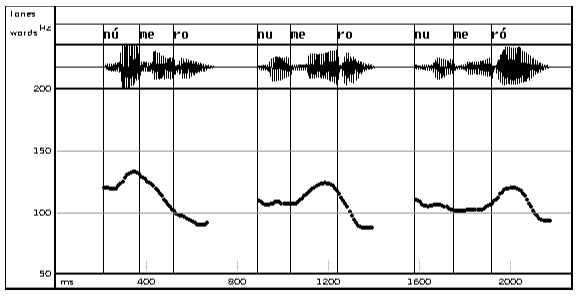
\includegraphics[width= 0.8\columnwidth]{Graphics/numero}
\caption{Pico en la t\'onica. Tomado de \cite[p.4]{hualde2003modelo}}
\label{numero}
\end{center}
\end{figure}




 Este modo de an\'alisis var\'ia de lengua a lengua tamb\'ien porque en algunas la melod\'ia tiene valor l\'exico: las llamadas lenguas tonales, como el mandar\'in. Para este tipo de lenguas se discute si es suficiente la definici\'on de solo tono alto y bajo ~($H$ y $L$). En las intonacionales, como el inglés o el español, la entonaci\'on no altera el significado de la palabra sino su valor pragm\'atico. En otros idiomas, como el sueco, la entonaci\'on tiene en parte funci\'on pragm\'atica y en parte, l\'exica \cite{hualde2003modelo}.

\subsection{Acentos tonales}
A la hora de transcribir un enunciado con el modelo AM lo primero que se debe conocer es la lengua. Para cada una se define un conjuto de acentos tonales espec\'ifico. En principio el sistema considera los siguientes acentos monotonales y bitonales:

\begin{comment}
En algunos idiomas se define un único acento tonal, por ejemplo para el japon\'es de Tokio solo existe H*+L. Para el inglés se ha propuesto un inventario con al menos 5 acentos tonales diferentes. 
\end{comment}

\begin{description} \label{tonos}
\item[H*] Pico en la tónica.
\item[L*] Valle en la tónica. 
Ejemplo: \emph{¿Me callo?} Se denotaría como L* H\% .El contorno entonativo en la s\'ilaba tónica “ca” recibe tono bajo por la interrogación y un ascenso al final de la frase.
\item[L+H*] Pico en la tónica precedido por un valle (subida de la pretónica a la tónica).
\item[L*+H] Valle en la tónica seguido por un pico (subida de la tónica a la postónica).
Ejemplo: \emph{Susana y Lucas se van ma\~nana.} (L*+H  L*+H  L+H*). Este tipo de acento es el que se observa en el espa\~nol en las palabras intermedias en las oraciones declarativas neutras sin \'enfasis especial en ninguna palabra. 
\item[H+L*] Valle en la tónica precedido por un pico (bajada de la pretónica a la tónica).
Ejemplo: \emph{Llegarán  ma\~nana.} (L*+H  H+L*  L\%).
\item[H*+L] Pico en la tónica seguido por un valle (bajada desde la tónica).
\end{description}



Con el conjunto de elementos contrastivos  definido, se detecta cada una de las s\'ilabas con acento l\'exico, solo las m\'as prominentes como se ha dicho antes, y se les asocia un acento tonal. Aunque lucen atractivas estas notaciones, es importante destacar lo confusa que resulta muchas veces y hasta entre los propios expertos, por ejemplo, al anotar un segmento espec\'ifico es debatible si ubicar un pico en la t\'onica o en la post\'onica \cite[p.72]{pierrehumbert1980phonology}.



\subsection{Tonos de frontera}

En el AM existen dos tipos de frases prosódicas: la frase entonativa y la frase intermedia. Una frase entonativa consiste en una o más frases intermedias. Al final de ambos tipos de frase podemos tener un tono de frontera.
Los tonos de frontera de frase entonativa se indican como L\%, H\%. Los tonos que marcan el final de una frase intermedia se señalan como L-, H-.

Ejemplo: \emph{¿Quieres ir a tomar helado o salir a caminar?} (H- H\%)

Esta frase entonativa contendría dos frases intermedias: “quieres ir a tomar helado” y “o salir a caminar”.



Se consideran los siguientes tonos de frontera:

\begin{description}
\item[L-L \%] Descenso final (final de oraciones declarativas).
\item[L-H\%] Descenso incompleto con subida de continuaci\'on al final.
\item[H-L\%] Suspensi\'on.
\item[H-H\%] Subida final (final de la interrogativa).
\end{description}


\begin{comment}
Se ha hablado tambi\'en de la necesidad de incluir acentos para los inicios de frase. Por ejemplo en espa\~nol las oraciones interrogativas tienen un comienzo relativamente m\'as alto que las declarativas.
\end{comment}




\subsection{Modelo ToBI}   \label{tobi}
En 1992 \cite{silverman1992tobi}, por el acuerdo entre varios especialistas y su intenci\'on de hacer una adaptaci\'on al ingl\'es del modelo AM nace el sistema ToBI~(TOnes and Break Indices). Este trata de aliviar los puntos flacos de la teor\'ia precedente\footnote{Existen muchos enfoques de an\'alisis diferentes, basta comparar una transcripci\'on con Tobi y otra con Todi ~(adaptaci\'on al holand\'es de AM) para ver lo mucho que distan a\'un cuando los contornos entonativos del ingl\'es y el holand\'es coinciden casi completamente \cite[p.23]{hualde2003modelo}.} y una de las modificaciones m\'as importantes que incluye es que permite la demarcaci\'on entre frases y palabras con la inclusi\'on de \'indices. Considera los mismos acentos tonales planteados inicialmente por AM excepto H*+L \cite{silverman1992tobi}. Se han implementado algoritmos para la anotaci\'on autom\'atica con TOBI, espec\'ificamente se puede hacer referencia a Autobi de 2010 \cite{rosenberg2010autobi}\footnote{\url{https://github.com/AndrewRosenberg/AuToBI}}.


\section{Sistema entonativo de Garc\'ia River\'on}
Similar al concepto de sintonema de Navarro, nace el de \emph{entonema}, definido por Garc\'ia River\'on como \cite{raquel2018interrogativa}:


\begin{quote}
``(...) la unidad entonativa formada por un haz de rasgos distintivos que se ordena en un eje paradigm\'atico, se realiza en un eje sintagm\'atico y cumple funciones comunicativas espec\'ificas en los actos del habla. Un cambio de \emph{entonema} puede ocasionar una ruptura de la cadena comunicativa en el texto.''
\end{quote}

La anotaci\'on por entonemas constituye un m\'etodo de transcripci\'on pros\'odica diferente: mientras que con ToBI la curva mel\'odica se reconstruye por los acentos tonales y tonos de frontera, cada entonema ya denota un comportamiento particular de la misma. A los segmentos de voz que para AM constityen frases intermedias es a los que se les asocia un tonema espec\'ifico.

Para el espa\~nol de Cuba\footnote{Espec\'ificamente el espa\~nol hablado en la capital, Ciudad de La Habana.}, la prestigiosa enton\'ologa Raquel Mar\'ia Garc\'ia River\'on ha estructurado y definido un \emph{sistema entonativo} representado por 18 entonemas principales:

\begin{description}
\item[E-1:]  Enunciaci\'on neutral. Es encontrado frecuentemente en las respuestas y en los segmentos de conclusi\'on.  
\item[VE-1a:]  Advertencia.
\item[ VE-1b:] Aclaraci\'on, evidencia. 
\item[ VE-1c:] Petici\'on marcada por un sentimiento de ruego. 
\item[ E-2:] Pregunta con alto grado de desconocimiento con respuesta argumentativa donde todos los elementos desconocidos son igualmente probables. Se considera la gran similitud que presenta con la enunciaci\'on neutral ~\cite[p.95]{garcia1996aspectos1}.
\item[ VE-2a:] Interrogaci\'on enf\'atica, con matiz categ\'orico.
\item[ E-3:] Interrogaci\'on con alto grado de desconocimiento con respuesta afirmativa o negativa.  Interrogativa absoluta.
\item[ VE-3a:] Preguntas con asombro o extrañeza. Expresan bajo grado de desconocimiento. Presentan similitud con algunas exclamaciones descritas por Antonio Quilis\footnote{Director del Laboratorio de Fon\'etica Experimental del Consejo Superior de Investigaciones Cient\'ificas de Madrid.} ~\cite[p.97, nota 13]{garcia1996aspectos1}.
\item[ VE-3b:] Interrogaci\'on de comprobaci\'on con baj\'isimo grado de desconocimiento. Corroboraci\'on, suposici\'on. Se encuentra muy cercano a la enunciaci\'on ~\cite[p.99]{garcia1996aspectos1}.
\item[ E-4:] Interrogaci\'on cuya inc\'ognita se expresa anteriormente en el di\'alogo o en el contexto. Se introducen con una \emph{Y} inicial.
\item[ VE-4a:] Interrogaci\'on inconclusa. 
\item[ E-5:] Delimitador de no conclusi\'on. Se plantea su gran similaridad con la curva de la interrogaci\'on absoluta ~\cite[p.104]{garcia1996aspectos1}. 
\item[ VE-5a:] Ejemplificador con alargamiento de la \'ultima s\'ilaba. 
\item[ VE-5b:] Argumentativa de no conclusi\'on con la cl\'ausula \emph{como}. Expresa causalidad.
\item[ E-6:] Ponderaci\'on, oraci\'on valorativa. Es una curva con terminaci\'on ascendente.
\item[ VE-6a:] Ponderaci\'on descendente. Respecto al \emph{entonema 6} no introduce valor comunicativo nuevo generalmente.
\item[ E-7:] Aperlativa.
\item[ VE-7a:] Aperlativa a distancia. 
\end{description}

Las caracter\'isticas ac\'usticas de estas categor\'ias fueron reveladas con un serio experimento en el Laboratorio de Fon\'etica Experimental del \emph{Instituto Pedag\'ogico de Lenguas Extranjeras} de Mosc\'u en el a\~no 1985 \cite{garcia1996aspectos2} y bajo la l\'inea de los \emph{rasgos distintivos}.
\begin{comment}
\subsection{Oposiciones}
Se pueden encontrar formas de entonar naturales, espont\'aneas y estimuladas psico1\'ogicamente; se utilizan formas con alguna intencionalidad y aparecen tambi\'en oposiciones en las cuales el valor psicofisiol\'ogico de la sustancia entonativa es irrelevante, por lo que entran dentro del sistema ling\"u\'istico de una lengua dada. \cite{garcia1996aspectos1}.


El contorno entonativo se puede segmentar cuando se establecen oposiciones.


Asi, a modo de ejemplo, se puede sefialar que el entonema E-l, que coincide con E-S por la forma, se diferencia de este, entre otros indicadores, por la figura del segmento poslonicO. La VE-2a coincide con E·t en la fanna, pero se diferencia de este por la figura del segmento postonico y por el nivel inicial del de la curva de enlonacion. 

\end{comment}


\subsection{Rasgos distintivos}
Garc\'ia River\'on define una serie de indicadores que permiten diferenciar los entonemas y que adem\'as tienen 
relevancia en el plano de la descripci\'on ling\"u\'istica y la funci\'on comunicativa \cite[ac\'apite 2.1.1]{garcia1996aspectos2}:
\begin{enumerate}
\item La forma
\item La figura
\item La cumbre tonal
\item El tiempo voc\'alico relativo
\item El tiempo voc\'alico m\'aximo
\item La intensidad m\'axima
\item La velocidad del fundamental
\item El registro
\item El diapas\'on
\end{enumerate}

\begin{comment}
Se ha comprobado la importancia de la forma (en relacion con el papel esencial que cum pie como rasgo diferencial de varias realidades acusticas), seguida por lafigura del segmento postonico, figura del centro de entonacion, nivel final y nivel de Fa maximo.


Es fici] de darse cuenta que, segun demuestra la somera resefia que he realizado del comportamiento de algunos de estos rasgos, fa productividad de los indicadores que nos ocupan puede variar dentro de un tipo u otro de investigacion. 


 No se descarta Ia posibilidad, ademas, de que sea necesario introducir otras tipos de indicadores 
\end{comment}

A estos les llama \emph{rasgos distintivos}. La diferenciaci\'on de los tonemas a partir de esa base, se refleja en las tablas \ref{rasgos_dist1} y \ref{rasgos_dist2}. Seg\'un la enton\'ologa, el indicador que mejor delimita los tonemas es la forma de la curva mel\'odica y es el \'unico rasgo en que se diferencian VE-1a, VE-1c, VE-2a, VE-3a, VE-3b y RE-6a~(ver Tabla \ref{rasgos_forma} anexada en el documento)  \cite[p.247]{garcia1996aspectos2}. Los siguientes par\'ametros m\'as discriminantes que declara~(ver anexo \ref{productividad}), son la figura del segmento post\'onico y el nivel final ~(regsitro).


\begin{description}
\item[La forma:] se refiere al tipo de curva que describe el movimiento de la \emph{F0}. Se detectan 4 patrones principales \emph{c\'oncava}, \emph{convexa}, \emph{recta} y \emph{zigzagueante}, incluidas tambi\'en todas sus combinaciones.
\item[La figura:] es el movimiento que realiza la curva mel\'odica dentro de una secuencia de hasta 3 s\'ilabas. Se diferencian 3 tipos: \emph{descendente}, \emph{ascendente} y \emph{llana}. Garc\'ia River\'on en su estudio, toma en cuenta este par\'ametro para el \emph{centro de la entonaci\'on} y el \emph{segmento post\'onico} \cite[p.214]{garcia1996aspectos2}.
\item[El registro o nivel del tono:] se puede determinar con la relaci\'on entre la frecuencia m\'axima y la m\'inima. En sus investigaciones, Garc\'ia River\'on analiza este par\'ametro aparejado tambi\'en a las frecuencias inicial y final.
\end{description}

\begin{comment}
rasgos mas discriminantes escalafon:
- forma
- nivel final (tercer lugar)
- diapason (4to lugar)
- nivel inicial: sirve para diferenciar ve-1c
- figura

- tiempo vocalico relativo (septimo lugar)
I. t = (Σti)/n   donde: t = media aritmética del corpus  Σ ti =  sumatoria de todos los tiempos absolutos   n=cantidad de sílabas del corpus 
II. t.voc.rel. = ti                           t


- velocidad de la f0 (octavo lugar)
- intensidad maxima (tiene baja productividad pero esta asociado a los matices afectivos)
\end{comment}





\begin{figure}
\begin{center}
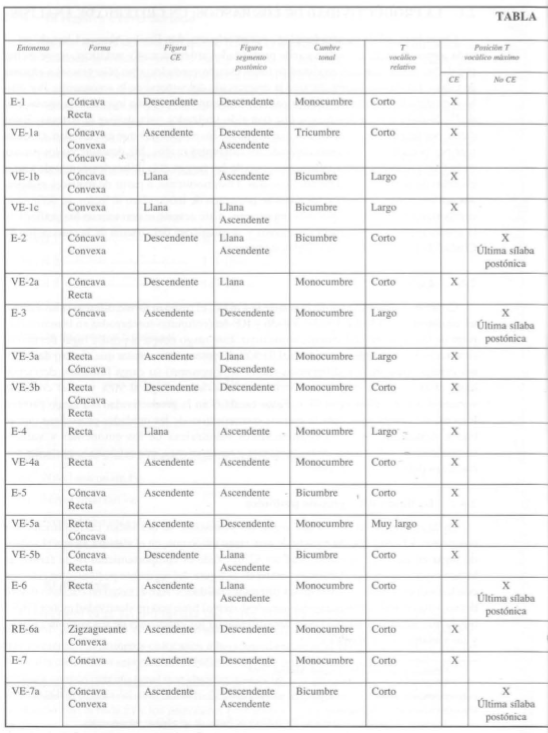
\includegraphics[width= 1\columnwidth]{Graphics/rasgos_dist1}
\caption{Rasgos distintivos por entonemas. Parte 1. Tomado de \cite[p.218]{garcia1996aspectos2}.}
\label{rasgos_dist1}
\end{center}
\end{figure}


\begin{figure}
\begin{center}
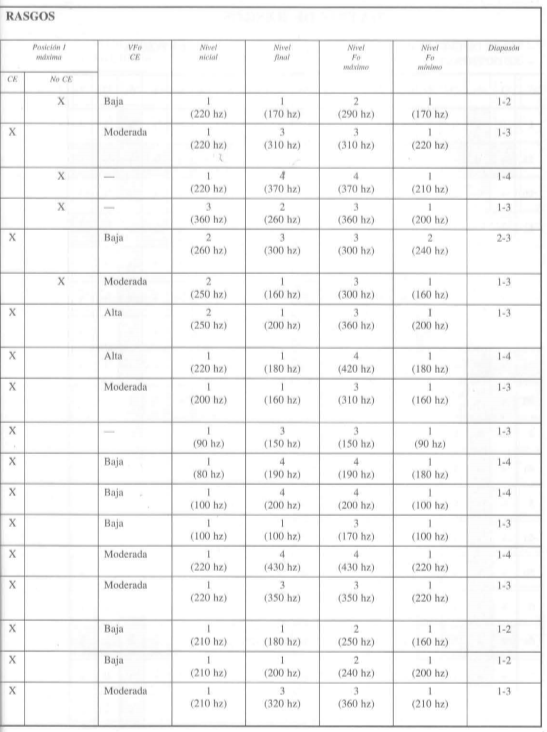
\includegraphics[width= 1\columnwidth]{Graphics/rasgos_dist2}
\caption{Rasgos distintivos por entonemas. Parte 2. Tomado de \cite[p.219]{garcia1996aspectos2}.}
\label{rasgos_dist2}
\end{center}
\end{figure}



\begin{comment}
aqui va la tablita

	\section{Comparaci\'on con sistema Tobi.}
	
	TOBI y el sistema propuesto por la doctora River\'on son ambos modelos de anotaci\'on pros\'odica solo que el primero anota por palabras y el segundo por frases. Los dos surgen para estudiar los elementos contrastivos del sistema mel\'odico~(ver tabla \ref{comparacion).
	
	\begin{table}
	\begin{center}
	\begin{tabular}{l|rr} 
	& \bf Sistema Tobi & \bf Sistema River\'on \\ \hline
	\bf Lengua    &   Ingl\'es  &    Espa\~nol de Cuba. Ciudad de La Habana   \\ 
	\bf A\~no en que se propone & 1992 & 1996 \\
	\bf M\'etodo & Transcribe por palabras cuya s\'ilaba t\'onica tiene mayor prominencia tonal y construye la curva mel\'odica con la interpolaci\'on de la combinaci\'on de los acentos tonales y tonos de frontera de dicha transcripci\'on & Anota por frases\footnote{Lo que en el sistema Tobi ser\'ia una frase intermedia} que ya tienen determinado un patr\'on de contorno mel\'odico \\
	\end{tabular}
	\caption{Comparaci\'on entre sistemas.}\label{comparacion}
	\end{center}
	\end{table}
\end{comment}


\section{Conclusiones}
Dado que ToBI y el sistema propuesto por la Dra.C. Garc\'ia River\'on son ambos modelos de anotaci\'on pros\'odica, aunque expresados en t\'erminos diferentes, se pudiera pensar que las herramientas que existen para anotar con ToBI son la soluci\'on de este problema. Esto se descarta recordando que:

\begin{enumerate}
\item La teor\'ia de Garc\'ia River\'on es antireduccionista, es decir, que apoya la idea de que no puede considerarse solo el comportamiento de la curva mel\'odica, sino tambi\'en otros rasgos como la intensidad, la duraci\'on y el timbre \cite{menendez2008estudio}.
\item Aunque algunos recursos para anotar con ToBI han sido adaptados al espa\~nol, puede que no sean efectivos con el espa\~nol de Cuba que, como bien se ha expuesto, tiene sus especificidades. Adem\'as se ha demostrado que un mismo contorno entonativo var\'ia de un hablante a otro ~(ver anexo \ref{diferencialocutor}); a\'un mayor debe ser la diferencia entre locutores de lenguas diferentes.
\end{enumerate}

\chapter{Fundamentaci\'on te\'orica} 
El germen de toda la metodolog\'ia planteada en esta investigaci\'on se basa en los estudios desarrollados 
por la doctora Raquel Garc\'ia River\'on y de manera muy especial, se apoya en los apuntes del segundo tomo de 
su trilog\'ia \emph{Aspectos de la entonaci{\'o}n hisp{\'a}nica}  \cite[cap\'itulo II]{garcia1996aspectos2} en el 
cual dedica un extenso apartado a los \emph{rasgos distintivos de la entonaci\'on}.

\section{Teor\'ia Wavelet} \label{wavelet_theory}
Como ha definido la Dra. Garc\'ia River\'on, el par\'ametro diferenciador m\'as fuerte entre los entonemas es la forma del movimiento de la F0. Uno de los modelos matem\'aticos que mejor puede capturar la descripci\'on de la forma de una curva es el m\'etodo de la \emph{Transformada Wavelet}~(WT, por sus siglas en ingl\'es, \emph{Wavelet Transform}), el cual funciona perfectamente para analizar se\~nales aperi\'odicas y con ruido\cite{addison2017illustrated}.


Al igual que la STFT propone una conversi\'on de la se\~nal al dominio tiempo-frecuencia \cite[p.99]{sundararajan2016discrete} obtiendo una representaci\'on m\'as \'util de la misma. Puede interpretarse como una convoluci\'on entre la se\~nal y un tipo especial de funci\'on: la wavelet~(ond\'icula).



En esencia, la Transformada Wavelet cuantifica cu\'an bien correlaciona la llamada \emph{wavelet madre} \cite[p.27]{debnath2002wavelet} con la se\~nal para cada par de valores de traslaci\'on y dilataci\'on\footnote{Las ond\'iculas pueden moverse a lo largo de la se\~nal y escalarse (estirarse o estrecharse).}. Toda esta informaci\'on se representa en el bidimensional \emph{plano de la transformada} \cite[p.3]{addison2017illustrated}.

\subsection{Ond\'iculas. Propiedades}
Una ond\'icula es una funci\'on localizada en el tiempo y con la forma de una peque\~na onda. Sea la funci\'on $\psi(t)$, se considera una wavelet si~\cite[p.10]{addison2017illustrated}:
\begin{enumerate}
\item Tiene energ\'ia finita, o sea cumple que:
	\begin{equation}\label{E:energy}
	E = \int_{-\infty}^{\infty} |\psi(t)|^{2} dt < \infty
	\end{equation}
	
\item Si 
	\begin{equation}\label{E:transwav}
	\hat{\psi}(f) = \int_{-\infty}^{\infty} \psi(t) e^{-i(2\pi f) t} dt
	\end{equation}
	es la transformada de Fourier de $\psi(t)$ entonces se cumple:
	
		\begin{equation}\label{E:admisibilidad}
		C_g = \int_{0}^{\infty} \dfrac{|\hat{\psi}(f)|^2}{f} df < \infty
		\end{equation}
	lo cual significa que $\psi(t)$ tiene media cero~($\hat{\psi}(0)=0$). A esta propiedad se le llama \emph{condici\'on de admisibilidad} ~\cite[p.11]{debnath2002wavelet} donde $C_g$ es conocida como la constante de admisibilidad y depende de la ond\'icula. 
\end{enumerate}

Existen otros requerimientos que deben considerarse para catalogar una funci\'on como ond\'icula pero son aplicados principalmente a las llamadas wavelets complejas\footnote{Las wavelets complejas son aquellas que tienen no s\'olo componente real, sino tambi\'en imaginaria. Una muy importante con esta condici\'on es la de \emph{Morlet}\cite[secci\'on 2.11]{addison2017illustrated}.}.


\subsection{Transformada Wavelet Discreta}
Sea la funci\'on wavelet $\psi(t)$ trasladada y dilatada:

$$ \psi_{a,b}(t) = \psi(\dfrac{t-b}{a})  $$

donde se dice que $a$ es el \emph{par\'ametro de dilataci\'on} y $b$ \emph{par\'ametro de traslaci\'on}. 


Esta expresi\'on representa el caso continuo de la transformada, puesto que los par\'ametros $a$ y $b$ toman todos los posibles  valores en los reales. 


Si solo se consideraran valores discretos de traslaci\'on y dilataci\'on entonces se habla de la Transformada Wavelet Discreta~(DWT, por sus siglas en ingl\'es, \emph{Discrete Wavelet Transform}).


Una ond\'icula $\psi(t)$ puede discretizarse mediante la f\'ormula:

\begin{equation}\label{E:discretizacion_a_b}
	\psi_{m,n}(t) = \dfrac{1}{\sqrt{a_{0}^m}}
	\psi(\dfrac{t - n b_{0}a_{0}^m}{a_{0}^m})
\end{equation}

donde:

\begin{enumerate}
\item  El entero $m$ controla la dilataci\'on.
\item  El entero $n$ controla la traslaci\'on.
\item $a_0$ es un par\'ametro de paso de dilataci\'on prefijado mayor que 1.
\item $b_0$ es el par\'ametro de localizaci\'on que debe ser mayor que 0.
\end{enumerate}

La DWT de una se\~nal continua $x(t)$ por tanto, se expresa mediante: 

\begin{equation}\label{E:trans_discreta}
	T_{m,n} = \int_{-\infty}^{\infty} x(t)
	\dfrac{1}{a_{0}^{m/2}}
	\psi(a_{0}^{-m}t - nb_0) dt
\end{equation}

que puede expresarse tambi\'en en t\'erminos del producto escalar:

\begin{equation}\label{E:trans_discreta_inner}
	T_{m,n} = \langle x, \psi_{m,n}  \rangle
\end{equation}

En la Transformada Wavelet Discreta los valores de $T_{m,n}$ son conocidos como \emph{coeficientes wavelets} o \emph{coeficientes de detalle}.
  
  \subsubsection{Reconstrucci\'on de la se\~nal. Dyadic Grid}
  
 La funci\'on $x(t)$ puede reconstruirse como:
   
   \begin{equation}\label{E:discrete_reconstrution}
   	x'(t) = \dfrac{2}{A + B}
   	\sum_{m=-\infty}^{\infty} 
   	\sum_{n=-\infty}^{\infty}
   	T_{m,n} \psi_{m,n}(t)
   \end{equation}
   
   donde $x'(t)$ es la reconstrucci\'on difiriendo de la se\~nal original, $T_{m,n} $  son los coeficientes de detalle y $A, B$ son par\'ametros del enfoque de Marcos de Wavelet\footnote{Permite determinar cu\'an buena es la representaci\'on de una se\~nal con DWT.} \cite{addison2017illustrated} \cite{debnath2002wavelet} que son elegidos convenientemente y dependen de los par\'ametros de dilataci\'on y traslaci\'on $a_0,b_0$. Si $A = B$, la reconstrucci\'on es exacta.
   
   
   
   Al aplicar \emph{Dyadic Grid}\footnote{Es muy com\'un que los valores de $a_0$, $b_0$ se prefijen como 2 y 1 respectivamente puesto que adem\'as de ser la forma de discretizaci\'on m\'as simple y eficaz, define una base de ond\'icula ortonormal. A este arreglo se le conoce como Dyadic Grid.} \cite{addison2017illustrated} la se\~nal puede ser reconstruida en t\'ermino de los coeficientes de detalle, puesto que $\{ \psi_{m,n}(t) \}$ es ahora una base ortonormal:
    
     \begin{equation}\label{E:discrete_reconstrution_dg}
      	x(t) = \sum_{m=-\infty}^{\infty} 
      	\sum_{n=-\infty}^{\infty}
      	T_{m,n} \psi_{m,n}(t)
      \end{equation}
      
      
\subsubsection{Funci\'on de escala. Representaci\'on multiresoluci\'on}
A las funciones ond\'iculas discretas ortonormalizadas con Dyadic Grid se les asocian \emph{funciones de escala} \cite[secci\'on 3.2.3]{addison2017illustrated} \cite{sundararajan2016discrete} \cite{debnath2002wavelet}. La funci\'on de escala est\'a relacionanda con la suavidad de la se\~nal y se expresa:

  \begin{equation}\label{E:scaling_function}
  	\phi_{m,n}(t) = 2^{-m/2}\phi(2^{-m}t - n)
  \end{equation}
  
  
  De la misma forma que existe la ond\'icula madre, an\'alogamente para las funciones de escala est\'a la \emph{funci\'on de escala padre} o  simplemete \emph{wavelet padre},  $\phi_{0,0}(t) = \phi(t)$, y cumple \cite{addison2017illustrated} \cite[p.377]{debnath2002wavelet}:
  
   \begin{equation}\label{E:p1sf}
    \int_{-\infty}^{\infty}	\phi_{0,0}(t) dt = 1
    \end{equation}
    
La convoluci\'on de la funci\'on de escala con la se\~nal produce los llamados \emph{coeficientes de aproximaci\'on} \cite{addison2017illustrated}:

 \begin{equation}\label{E:scala_conv}
     	S_{m,n} = \int_{-\infty}^{\infty}
     	x(t) \phi_{m,n}(t) dt
 \end{equation}


Se puede obtener una \emph{aproximaci\'on continua} de la se\~nal de escala $m$ de la siguiente manera:

 \begin{equation}\label{E:aproximaccion_continua_m}
 x_m(t) = \sum_{n=-\infty}^{\infty}
     	S_{m,n} \phi_{m,n}(t)
 \end{equation}
 
 donde $x_m(t)$ es una versi\'on de la se\~nal original que depende de la funci\'on de escala \'indice $m$.
 
 Finalmente, la se\~nal puede reconstruirse a partir una aproximaci\'on continua mejorada con los coeficientes de detalle:
 
 \begin{equation}\label{E:rec_ca_cd}
 x(t) = x_{m_0}(t) +
     	\sum_{m=-\infty}^{m_0} d_m(t)
 \end{equation} 
 
 
 donde $m_0$ es un \'indice de escala arbitrario y $d_m(t)$ es conocido como \emph{detalle de la se\~nal} y se expresa:
 
 \begin{equation}\label{E:signal_detail}
  d_m(t) = \sum_{n=-\infty}^{\infty}
   	T_{m,n}\psi_{m,n}(t)	
 \end{equation} 
 
 De la ecuaci\'on \ref{E:rec_ca_cd} se deslinda f\'acilmente lo que se conoce como \emph{representaci\'on multiresoluci\'on}:
 
 \begin{equation}\label{E:multiresolution_representation}
   x_{m-1}(t) = x_{m}(t) + d_m(t)
  \end{equation} 
  
  
  Esta propiedad es una de las m\'as atractivas de la Teor\'ia Wavelet y sus aplicaciones son dis\'imiles \cite{barba2011reconocimiento, cano2010analisis}.
 

\section{Aprendizaje autom\'atico}
El enfoque de tratamiento m\'as fuerte con que se ha enfrentado el problema ha sido el Aprendizaje Autom\'atico~(ML, por sus siglas en ingl\'es, \emph{Machine Learning}). De manera espec\'ifica se propone la variante de \emph{aprendizaje supervisado} puesto que, aunque son complejos, se conocen los criterios que permiten discriminar entre los datos para asociarle una u otra categor\'ia, las cuales tambi\'en han sido previamente definidas.


Se trata de aprendizaje supervisado \cite[p.695]{russell2002artificial} cuando se tiene como entrada del algoritmo un \emph{conjunto de entrenamiento}, sea la sucesi\'on $\{ ((x^{(i)}, y^{(i)})\}$, y se espera conocer la funci\'on $f$ mediante la cual se produce la asociaci\'on $x\Rightarrow y$\footnote{Cada elemento $x$ se expresa por un juego de caracter\'isticas alineadas $x = [x_0,x_1,...,x_n]$, donde $n$ es fijo para un conjunto de entrenamiento dado.}. La funci\'on $h_\theta(x)$, referida como \emph{hip\'otesis}, se define para aproximar a $f$. Los par\'ametros $\theta = [\theta_0, \theta_1, ..., \theta_n]$ se ajustan para encontrar la hip\'otesis que mejor refleja la naturaleza del problema y se hallan resolviendo el problema de optimizaci\'on asociado a la minimizaci\'on de la llamada \emph{funci\'on de costo} $J(\theta)$ que cuantifica el error de la predicci\'on de un modelo sobre un determinado conjunto. $J(\theta)$ tiene la forma:

$$ J(\theta) = \dfrac{1}{2m} \sum\limits_{i=1}^{m} (h_{\theta}(x^{(i)}) - y^{(i)})^2 $$

 donde $x^{(i)}$ es el $i$-\'esimo elemento del conjunto de tama\~no $m$ para el cual el clasificador predice la etiqueta $y^{(i)}$.


Los clasificadores utilizados en la experimentaci\'on han sido: 
 \begin{description}
 \item[Regresi\'on Log\'istica:] Etiqueta los elementos con un umbral de clasificaci\'on \cite{murphy2012machine}. Su hip\'otesis plantea:
 \begin{equation}\label{E:logistic_regression_hipotesis}
 h_\theta(x) = \dfrac{1}{1 + e^{-\theta^Tx}}
 \end{equation}
 \item[SVM:] Las M\'aquinas de Soporte Vectorial~(SVM, por sus siglas en ingl\'es, \emph{Support Vector Machine}) surgen 1963  por iniciativa de Vladimir N. Vapnik y Alexei Ya. Chervonenkis en la Uni\'on Sovi\'etica. 
 Su hip\'otesis discrimina los datos con la construcci\'on de un hiperplano lineal que maximiza la distancia m\'inima posible entre los elementos. Incluye el uso de funciones de \emph{kernel} para la b\'usqueda del plano separador en una mayor dimensi\'on de los datos si es necesario \cite[p.15]{francois2017deep} \cite{duda2012pattern}.
 \end{description}




\begin{comment}
\subsection{Curva de aprendizaje, matriz de confusi\'on}
\subsection{M\'etricas}
\subsubsection{Validaci\'on cruzada}
\subsubsection{Presici\'on, recobrado y medida f0.}


\subsection{Feature selection}
\subsection{Correlation, anova test, feature importance}
\subsection{Dataset balanceado}
\subsection{Overfitting y underfitting}
\end{comment}




\section{Descriptores de la curva} 
\subsection{Convoluci\'on linear}

La \emph{convoluci\'on} es una operaci\'on mediante la cual se obtiene una funci\'on que representa la suma de superposici\'on entre una funci\'on $f$ y la versi\'on trasladada e invertida de otra funci\'on $g$.


Para el caso discreto la \emph{convoluci\'on}\footnote{ \url{https://mue.music.miami.edu/thesis/jvandekieft/jvchapter2.htm, https://ccrma.stanford.edu/~jos/Misc/Linear_Convolution_finite_length.html}).}  puede calcularse como:

$$ (f*g)[n] = \sum\limits_{k=0}^{N-1} f[k]g[n-k]$$


Se hace la distini\'on de linear, puesto que tambi\'en existe la convoluci\'on circular que se calcula:
 $$ (f \circledast g)[n] = \sum\limits_{k=0}^{N-1} f[k]g[n-k]_N$$ 
 
 donde $[n-k]_N$ significa $(n-k)$ m\'odulo $N$

\subsection{Entrop\'ia}
La \emph{entrop\'ia}\footnote{Teor\'ia de la informaci\'on de Shannon.} \cite{addison2017illustrated} \cite[p.703]{russell2002artificial} es una importante medida de informaci\'on  y cuantifica la incertidumbre de una \emph{variable aleatoria}. Para una muestra discreta $p = [p_1, p_2, ..., p_n]$ puede ser calculada como: 

   $$ S(p) = -\sum_{i=0}^n p_i log_2(p_i) $$
   
Un valor peque\~no de entrop\'ia indica alto contenido de informaci\'on. 

\subsection{Pendiente}
Tradicionalmete se habla de la \emph{pendiente} de una recta como una medida de su inclinaci\'on respecto a la horizontal. Para el caso de una curva $f(x)$ arbitraria, pudiera ser considerada como $n$ en la expresi\'on: $$F(x) = nx + n_0$$ donde
$F(x)$ es una aproximaci\'on  por \emph{m\'inimos cuadrados} \cite[p.59]{gautschinumerical} de $f(x)$ de grado 1 con funciones base polin\'omicas. 


\subsection{Espectro de potencias}
 Sea $f$ una se\~nal peri\'odica, a la sucesi\'on ${\hat{f}_0}^2, {\hat{f}_1}^2, ..., {\hat{f}_n}^2$ se le llama \emph{espectro de potencias} o simplemente \emph{espectro} \cite{hansen2014fourier}, donde $\hat{f}$ son los coeficientes de la \emph{transformada discreta de Fourier}. Tambi\'en puede calcularse solo como $\{|\hat{f}_i|\}$. Da la medida de cu\'anto hay de cada frecuencia en la se\~nal.

\section{Aumento de Datos} \label{aumento}
La aplicaci\'on de Aprendizaje Autom\'atico, de manera general, requiere el uso de grandes cantidades de datos
para entrenar y sobre todo en los casos en los que se han considerado tantos par\'ametros para caracterizarlos. Desafortunadamente, es com\'un que se cuente solo con un corpus peque\~no y que adem\'as sea complicado construir datos nuevos para enriquecerlo.  


Por este motivo, nace la t\'ecnica de \emph{Aumento de Datos}~(DA, por sus siglas en ingl\'es, \emph{Data Augmentation}) \cite{imai2005bayesian, hernandez2018data} que permite generar muestras artificiales a partir de diversas transformaciones aplicadas sobre otras generadas naturalmente. Usualmente es utilizada para aumentar el conjunto de entrenamiento. Ha sido llevada al campo del Procesamiento de Im\'agenes, el Reconocimiento Autom\'atico de Voz (ASR, por sus siglas en ingl\'es, \emph{Automatic Speech Recognition}) y hasta a la producci\'on y an\'alisis musical \cite{mcfee2015software, bhardwajaudio}.



Las transformaciones aplicadas dependen del objeto a sintetizar. En el Aumento de Datos para las im\'agenes, por ejemplo, lo que m\'as se utiliza es la rotaci\'on, el acercamiento(\emph{zoom}) y la traslaci\'on\cite{xue2016cnn, kim2020deepcapture}. En el caso de segmentos de voz la operaciones son otras. Se pueden tomar de ejemplo las siguientes que en adici\'on fueron las aplicadas en el experimento. Cada una fue producida con par\'ametros aleatorios.


Sea $\{x_i\}, i \in [1, N], i \in \mathbb{Z}$ la sucesi\'on que representa la se\~nal digital del audio de entrada:
\begin{enumerate}
\item Mezclar con otro sonido arbitrario que sirva de fondo. Esencialmente se produce con la suma $\{x_i + x_n\}$ donde $\{x_n\}$ es la sucesi\'on de la se\~nal que representa el ruido modificada a conveniencia.
\item Mezclar con peque\~nos  sonidos entre los cuales existen pausas arbitrarias. Se utiliza particularmente para cuando el segmento de audio original no tiene ruido y se desea simular un contexto en el que a veces se escuchan sonidos cortos de fondo.
\item A\~nadir ruido gaussiano\footnote{\url{https://www.researchgate.net/post/What_is_the_difference_between_Gaussian_noise_and_Random_Valued_Impulse_Noise}} a la muestra. Este tipo de ruido se produce con  distribuci\'on normal o gaussiana \cite{ross2009first}, que se denota como $X \sim N(\mu, \sigma^2)$ donde $\mu$ es la media y $\sigma^2$ es la varianza.
\item A\~nadir ruido gaussiano con SNR~(por sus siglas en ingl\'es, \emph{Signal to Noise Ratio})\footnote{\url{https://en.wikipedia.org/wiki/Signal-to-noise_ratio}} que es una medida muy utilizada en diversos campos como la medicina, la econom\'ia y la biolog\'ia pero en este caso se utiliza para comparar la amplitud de la se\~nal con el ruido de fondo \cite{thangjai2019confidence}.
\item Producir la convoluci\'on del audio con un IR~(por sus siglas en ingl\'es, \emph{Impulse Response})\footnote{\url{http://tulrich.com/recording/ir_capture/, https://ccrma.stanford.edu/~jos/filters/Impulse_Response_I_I.html}} arbitrario.
\item Ocultar una banda de tiempo del segmento de audio \cite{park2019specaugment}.
\item Ocultar una banda de frecuencia en el espectrograma del audio \cite{park2019specaugment}. 
\item Trasladar las muestras hacia adelante o hacia atr\'as con $k$ pasos\footnote{Casi exactamente la operaci\'on que se produce con \textit{numpy.roll()} de Python.}. Si $k>0$ entonces se obtiene $\{x_{N-k+1}\cdots x_N, x_1\cdots x_{N-k}\}$. Si $k<0$ entonces el resultado es $\{x_{|k|+1}\cdots x_N, x_1\cdots x_{|k|}\}$. Esta operaci\'on cuenta con el par\'ametro \textit{rollover} a partir del cual se deriva una versi\'on m\'as: si \textit{rollover == False} se igualan a cero los primeros $k$ lugares si $k>0$, si de lo contrario $k<0$, se igualan a cero los \'ultimos $k$ lugares.
\item Dilatar o acortar el tiempo de la se\~nal sin alterar el movimiento de la \emph{frecuencia fundamental} \cite{lu2017bidirectional, bhardwajaudio}.
\item Trasladar la \emph{curva mel\'odica} $n$ pasos sin afectar el tiempo \cite{bhardwajaudio}. Para lograr este efecto se han probado varias t\'ecnicas \cite{sturm2006pitch} desde enfoques con la \emph{Transformada de Fourier} hasta el uso de Constant Q -- Transform \cite{schorkhuber2012pitch}.
\item Considerar m\'as o menos puntos para representar la se\~nal~(upsampling\cite[ac\'apite 4.6.2]{oppenheim2001discrete}, downsampling\cite[ac\'apite 4.6.2]{oppenheim2001discrete}, respectivamente).
\item Distorcionar la se\~nal nivelando un porcentaje de puntos arbitrario, es decir, dado el porciento se determina un intervalo, sea $[a,b]$ y todos los valores fuera de \'el se igualan a los l\'imtes del mismo: todo $x_j, j < a$ se iguala a $x_a$ y todo $x_j, j>b$ se iguala a $x_b$. Tal porciento es tomado de una distribuci\'on uniforme. Los \'indices $\{a,b\}$ tambi\'en pueden ser negativos.
\item Normalizar la muestra, o sea, se obtiene la sucesi\'on $\left\{ \dfrac{x_i}{x_{max}}  \right\}$ donde $x_{max} = max(\{x_i\})$. Los nuevos valores se ubican en el rango de $[1,-1]$.
\end{enumerate}
\chapter{Experimentaci\'on y Resultados}\label{chapter:resultados}
Todo el proceso de experimentaci\'on y los resultados logrados fueron por v\'ia del lenguaje de programaci\'on Python y sus bibliotecas. 

\section{Creaci\'on del corpus}

Para este problema, como bien se ha dicho, las investigaciones son casi nulas desde el punto de vista computacional, y como una de las consecuencias, no existen corpus grandes anotados, por ende fue necesario construir uno. 

En el trabajo con Aprendizaje Autom\'atico casi siempre la mirada gira en torno a la comparaci\'on entre los clasificadores y la b\'usqueda de las caracter\'isticas correctas para describir los elementos, y se asume que existe un juego de datos ideal para la corrida del algoritmo. Al menos este no ha sido el caso y evidencia lo complicada que es esta fase de la experimentaci\'on.

Inicialmente, se contaba con una pequeña muestra de tamaño 42, anotada por los ling\"uistas, con menos de 7 ejemplares por entonema. A partir de \'el se produjeron las grabaciones finales con un total de 271 audios, 7 a 27 muestras por clase y generados por un locutor de g\'enero femenino. La descripci\'on se muestra bien detallada en la Tabla \ref{Ta:tablita}. Es necesario no dejar pasar por alto lo ambig\"ua que llega a ser la anotaci\'on para alguien que no es especialista, puesto que como mismo algunos entonemas resultan inconfundibles, tales como el 6 y el 5b, por el papel tan especialmente expresivo que tienen en el habla coloquial de Cuba, otros no dejan l\'imites muy claros, tal es el caso de los entonemas 2 y 3 que expresan igualmente interrogaci\'on con alto grado de desconocimiento y deslindado solo por el tipo de respuesta, o tambi\'en, el caso del entonema 4, las preguntas que comienzan con \emph{Y}. La diferenciaci\'on de estas 3 categor\'ias, por ejemplo, es singularmente sutil desde un an\'alisis entonol\'ogico.

\begin{table}
\begin{center}
\begin{tabular}{l|r} \hline
\bf Entonema & \bf Cantidad de muestras \\ \hline
 1 & 25 \\ 
 1a & 16 \\ 
 1b & 27 \\ 
 1c & 18 \\ 
 2 & 14 \\ 
 2a & 23 \\ 
 3 & 26 \\ 
 3a & 15 \\ 
 3b & 7 \\
 4 & 11 \\
 4a & 17 \\
 5 & 12 \\
 5a & 11 \\
 5b & 10 \\
 6 & 10 \\
 6a & 10 \\
 7 & 7 \\
 7a & 12 \\ \hline
 
\end{tabular}
\caption{Muestras por entonema del corpus.}\label{Ta:tablita}
\end{center}
\end{table}




\subsection{Criterios para etiquetar el corpus}

Se consideraron los 18 entonemas estudiados e identificados por Garc\'ia River\'on. La anotaci\'on del corpus se produjo seg\'un las descripciones de la enton\'ologa para cada categor\'ia y con ayuda de las muestras iniciales para los casos menos evidentes.


\subsection{Aumento de datos} 
Puesto que 271 sigue siendo una cantidad pequeña para dar soluci\'on a este problema, fue necesario entonces el uso de \emph{aumento de datos}, lo cual se logr\'o por medio de la biblioteca \texttt{audiomentations}\footnote{\url{https://github.com/iver56/audiomentations}} de Python, aunque existen otras con la misma finalidad. De las transformaciones disponibles se aplicaron 14, que operan como las explicadas en \ref{aumento}.

\begin{comment}
\begin{enumerate}
\item TimeMask
\item FrequencyMask
\item AddGaussianSNR
\item PitchShift
\item TimeStretch
\item AddGaussianNoise
\item Shift
\item Shift without rollover
\item AddImpulseResponse
\item Resample
\item ClippingDistortion
\item AddBackgroundNoise
\item AddShortNoises
\end{enumerate}
\end{comment}


Para formar el conjunto \texttt{Test} se apartaron 2 de las grabaciones por entonema y las 14 transformaciones de cada uno, mientras que para el corpus final se conservaron las grabaciones restantes y el augmentation de 5 elegidas por entonema con 5 variantes por cada transformaci\'on. Se debe considerar que algunos de los audios aumentados fueron despreciados. Todas estas anotaciones quedan reflejadas con detalle en la tabla \ref{Ta:ct}.


\begin{table}
\begin{center}
\begin{tabular}{l|r|r} \hline
\bf Entonema & \bf Cant. muestras. Corpus. & \bf Cant. muestras. Conjunto Test \\ \hline
 1 & 371 & 30 \\ 
 1a & 363 & 28 \\ 
 1b & 372 & 30 \\ 
 1c & 365 & 30 \\ 
 2 & 361 & 29 \\ 
 2a & 367 & 28 \\ 
 3 & 372 & 30  \\ 
 3a & 362 & 30 \\ 
 3b & 355 & 29 \\
 4 & 355 & 29 \\
 4a & 363 & 30 \\
 5 & 357 & 30 \\
 5a & 355 & 30 \\
 5b & 356 & 30 \\
 6 & 354 & 30 \\
 6a & 356 & 30 \\
 7 & 350 & 29 \\
 7a & 355 & 29 \\ \hline
 Total & 6489 & 531 \\ \hline
\end{tabular}
\caption{Muestras por entonema del corpus final.}\label{Ta:ct}
\end{center}
\end{table}


\subsection{Vectorizaci\'on de la muestra}
Cada audio de entrada es caracterizado para su posterior clasificaci\'on por medio de:

\begin{description}
\item[cD:] Los coeficientes de detalle de la curva mel\'odica en el nivel 4 de descomposici\'on de la Transformada Wavelet Discreta con la base wavelet \emph{Daubechies}\cite{daubechies1992cbms}. En promedio, para los audios del corpus, tienen tama\~no 40.
\item[espectrum:] El espectro de potencias de la curva. Tiene dimensi\'on 300 en promedio.
\item[pendiente:] La pendiente del \emph{pitch} en s\'i mismo. Es un escalar.
\item[entrop\'ia:] Se consideran la del \emph{pitch} y la de los coeficientes de detalle.
\item[convoluci\'on:] Convoluci\'on linear discreta entre la curva mel\'odica y la reconstrucci\'on de la misma que se logra con los \emph{cD} del primer nivel en la descomposici\'on con DWT. Es un escalar\footnote{El primer valor de aplicar \texttt{scipy.signal.convolve()} como se explica en las \emph{Especificaciones de la implementaci\'on}.}.
\item[frecuencias:] Se consideran la frecuencia m\'axima, m\'inima, inicial y final de la curva mel\'odica. Estas caracter\'isticas son para representar el rasgo de \emph{registro}, se\~nalado por Garc\'ia River\'on.
\end{description}

\subsection{Peque\~nas especificaciones sobre la implementaci\'on}
La implementaci\'on fue desarrollada completamente con el lenguaje de programaci\'on Python:

\begin{enumerate}
\item Las grabaciones de los entonemas se codificaron en formato \texttt{.wav}.

\item La extracci\'on de la curva mel\'odica de cada segmento de audio se produjo con \texttt{amfm\_decompy.pYAAPT()}\footnote{\url{https://pypi.org/project/AMFM-decompy/}} que es una versi\'on para Python del algoritmo descrito en \emph{Yet Another Algorithm for Pitch Tracking} \cite{kasi2002yet}.

\item El trabajo con wavelets se desarroll\'o con \texttt{pyw}\footnote{\url{https://pywavelets.readthedocs.io/en/latest/}}: la DWT espec\'ificamente con, \texttt{pyw.dwt()} y la reconstrucci\'on de la se\~nal a partir de los coeficientes de detalles y de aproximaci\'on de cierto nivel, con \texttt{pyw.waverec()}.

\item La transformada discreta de Fourier se obtuvo con \texttt{numpy.fft.fft()}. Para hallar el espectro se utiliz\'o la variante de los m\'odulos.

\item La entrop\'ia se calcul\'o con un m\'etodo simple implementado por el autor.

\item La pendiente se determin\'o por medio de \texttt{numpy.polyfit()}.

\item El valor de convoluci\'on es el primero de la muestra discreta de tama\~no 2 que devuelve \texttt{scipy.signal.convolve()} con el par\'ametro \texttt{mode = "valid"}.

\item La manipulaci\'on y almacenamiento de los datos se produjo con \texttt{pandas}\footnote{\url{https://pandas.pydata.org/}}.

\item Todo el trabajo con Aprendizaje Autom\'atico se desarroll\'o con \texttt{sklearn} \cite{garreta2013learning}: los clasificadores SVM y regresi\'on log\'istica con \texttt{sklearn.svm.SVC} y \texttt{sklearn.linear\_model.LogisticRegression} y para el an\'alisis de los modelos se emple\'o \texttt{sklearn.model\_selection} y \texttt{sklearn.metrics}. 
\end{enumerate}






\subsection{Preprocesamiento}
Para la extracci\'on de caracter\'isticas de la curva mel\'odica se experimentaron dos preprocesamientos fundamentales:

\begin{description}
\item[Remover silencios:] Eliminar los valores iguales a cero del inicio y final de la curva.
\item[Corregir discontinuidad:] Se rellenan los silencios intermedios del \emph{pitch} estimando los valores que tomar\'ia si fuesen distintos de cero por medio de interpolaci\'on. 
\end{description}

Los resultados expuestos en la siguiente secci\'on solo tienen aplicado el primero de estos preprocesamientos, puesto que el segundo luce muy prometedor, pero en la pr\'actica solo reduce la puntuaci\'on de los clasificadores.

\section{Resultados}
Los clasificadores que esencialmente se aplicaron fueron \emph{SVM} y \emph{Regresi\'on Log\'istica}. Para estimar el sesgo y la varianza de cada clasificador se aplic\'o validaci\'on cruzada\footnote{Los resultados expuestos se produjeron con \texttt{sklearn.model\_selection.ShuffleSplit}~ (\url{https://scikit-learn.org/stable/modules/generated/sklearn.model_selection.ShuffleSplit.html})} con raz\'on de $60\%$ para entrenar $40\%$ para validar y 30 repeticiones. Las curvas de aprendizaje\cite[secci\'on 7.5.4]{murphy2012machine} sirvieron para detectar la presencia o no de \emph{overfitting} \cite[p.22]{murphy2012machine}.

\subsection{Experimento 1}
Las muestras de audio fueron vectorizadas 
considerando todas las cararacter\'isticas 
descritas 
en la secci\'on anterior. Los 
resultados\footnote{Los modelos fueron validados
 atendiendo a la 
medida accuracy y la varianza\cite{murphy2012machine}.} 
se reflejan en la Tabla \ref{r1} y 
las curvas de aprendizaje en las Figuras \ref{calr1} y \ref{casvm1}.



\subsection{Experimento 2}
Los audios se vectorizaron igualmente que como en el experimento 1, excepto que se prescindi\'o de los valores del espectro, por tanto se alcanza una reducci\'on considerable de la dimensi\'on del problema\footnote{De 433 caracter\'isticas se comienza a trabajar solo con 41.} para tratar de evadir el efecto de \emph{overfitting}. Los resultados se reflejan en la Tabla \ref{r2} y las curvas de aprendizaje en las Figuras \ref{carl2} y \ref{casvm2}.


\begin{figure}
\begin{center}
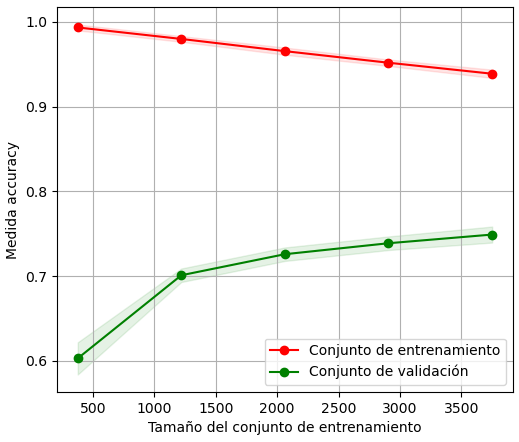
\includegraphics[width= 0.5\columnwidth]{Graphics/1}
\caption{Curva de aprendizaje con Regresi\'on Log\'istica. Experimento 1.}
\label{calr1}
\end{center}
\end{figure}

\begin{figure}
\begin{center}
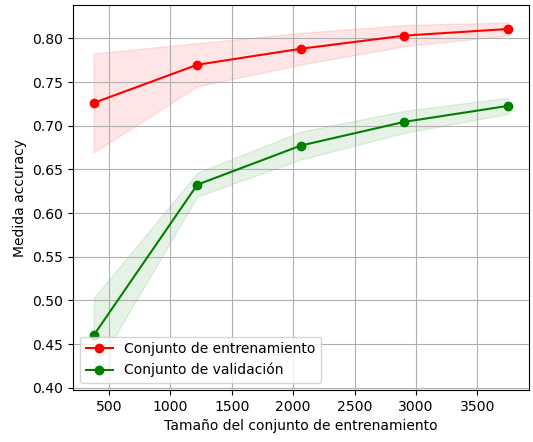
\includegraphics[width= 0.5\columnwidth]{Graphics/2}
\caption{Curva de aprendizaje con SVM. Experimento 1.}
\label{casvm1}
\end{center}
\end{figure}

\begin{table}
\begin{center}
\begin{tabular}{l|r|r} 
   & \bf Medida accurracy & \bf Varianza \\ \hline
 \bf SVM & 0.72 & 0.01 \\ 
 \bf Regresi\'on Log\'istica & 0.74 & 0.01 \\ 
\end{tabular}
\caption{Resultados de la validaci\'on cruzada. Experimento 1.}\label{r1}
\end{center}
\end{table}

\begin{figure}
\begin{center}
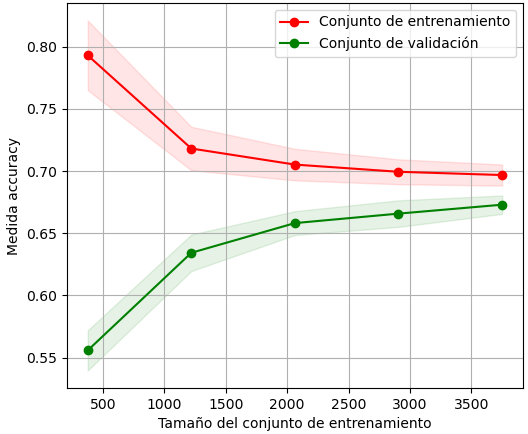
\includegraphics[width= 0.5\columnwidth]{Graphics/3}
\caption{Curva de aprendizaje con Regresi\'on Log\'istica. Experimento 2.}
\label{carl2}
\end{center}
\end{figure}

\begin{figure}
\begin{center}
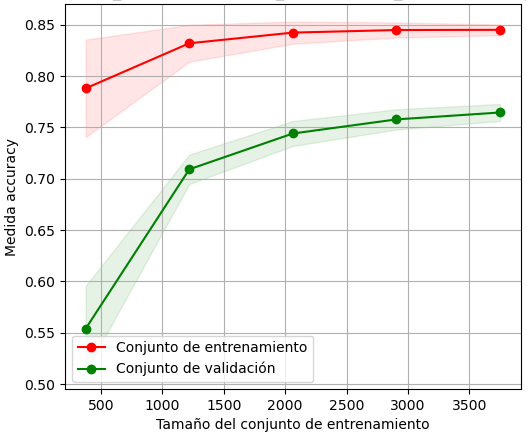
\includegraphics[width= 0.5\columnwidth]{Graphics/4}
\caption{Curva de aprendizaje con SVM. Experimento 2.}
\label{casvm2}
\end{center}
\end{figure}

\begin{table}
\begin{center}
\begin{tabular}{l|r|r} 
   & \bf Medida accurracy & \bf Varianza \\ \hline
 \bf SVM & 0.76 & 0.01 \\ 
 \bf Regresi\'on Log\'istica & 0.67 & 0.01 \\ 

\end{tabular}
\caption{Resultados de la validaci\'on cruzada. Experimento 2.}\label{r2}
\end{center}
\end{table}

\subsection{Evaluaci\'on en el conjunto \texttt{Test}}
Se elige el clasificador SVM del Experimento 2, pues presenta mayor puntaci\'on, su curva no indica presencia de \emph{overfitting} y considera menos caracter\'isticas. Los resultados\footnote{El an\'alisis se produjo antendiendo a la presici\'on, el recobrado y la medida-f1\cite{murphy2012machine,bay2009evaluation}.} de su evaluaci\'on en el conjunto \texttt{Test} se muestran en la Tabla \ref{test_result} y la Figura \ref{mcsvm2}. Se observa que la predicci\'on es nula para los entonemas VE-2a, VE-3a, E-5, VE-5a, VE-5b y E-6. Aunque no son buenas noticias, no indica necesariamente que el modelo sea incapaz siempre de predecir correctamente estas categor\'ias, recordando que, el conjunto \texttt{Test} es el \emph{Data Augmentation} de solo dos ejemplos por entonema.
\begin{table}
\begin{center}
\begin{tabular}{l|rrrr} 
& \bf precisi\'on & \bf recobrado & \bf medida-F1 & \bf   cantidad \\ \hline
         \bf 1 &       0.39  &    0.83  &    0.53   &     30 \\ 
         \bf 1a  &     0.16  &    0.32  &    0.21  &      28 \\
         \bf 1b    &   0.30   &   0.77 &     0.43    &    30 \\
         \bf 1c  &     0.52   &   0.80   &   0.63    &    30 \\
         \bf  2    &   0.17   &   0.14   &   0.15   &     29 \\
         \bf 2a     &  0.00  &    0.00   &   0.00    &    28 \\
        \bf   3   &    0.43  &   0.30  &    0.35  &      30 \\
        \bf  3a  &     0.00 &   0.00  &    0.00  &      30 \\
         \bf  3b  &     0.44 &   0.66  &    0.53    &    29 \\
       \bf   4   &    0.09  &   0.14  &    0.11     &   29 \\
       \bf  4a  &    0.23  &   0.10  &    0.14     &   30 \\
      \bf  5   &    0.00  &   0.00  &    0.00      &  30 \\
      \bf  5a  &     0.00 &   0.00  &    0.00     &   30 \\ 
     \bf   5b  &     0.00 &   0.00  &    0.00     &   30 \\
    \bf    6     &  0.00    &  0.00   &   0.00   &     30 \\
    \bf  6a     &  0.14    &  0.10   &   0.12    &    30 \\
     \bf    7     &  0.31    &  0.17   &   0.22     &   29 \\
   \bf  7a     &  0.57    &  0.45   &   0.50     &   29 \\ \hline
          \bf Medida accuracy     &          &         &  0.27     &  531 \\

\end{tabular}
\caption{Evaluaci\'on en el conjunto \texttt{Test}. Experimento 2. SVM.}\label{test_result}
\end{center}
\end{table}

\begin{figure}
\begin{center}
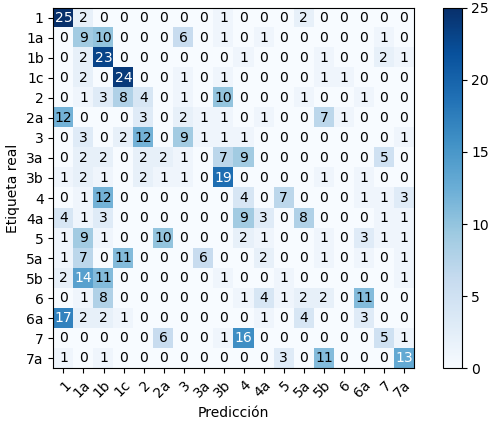
\includegraphics[width= 0.5\columnwidth]{Graphics/5}
\caption{Matriz de confusi\'on. Evaluado en conjunto \texttt{Test}. SVM Experimento 2.}
\label{mcsvm2}
\end{center}
\end{figure}

\begin{comment}
Raquel dice:
Segun estos indicadores, se pudo comprobar que las variantes VE-Ia, VE-lc, VE-2a, VE-3a. VE-3b y RE-6a se diferencian par un rasgo unico: la forma. Se ha observado que el rasgo mas productiv~ en este sentido es precisamente la forma del contamo mel6dico. 
- el diapason es importante
\end{comment}


\section{Software}
El producto final es un software que grafica el espectrograma de un audio de entrada y predice el entonema presente. La interfaz gr\'afica se produjo con la biblioteca \texttt{PyQt5} de Python y est\'a reflejada en las Figuras \ref{software} y \ref{software2} de los anexos.

\backmatter

\chapter*{Conclusiones}\label{chapter:conclusiones}
Se observ\'o finalmente, que el aprendizaje autom\'atico arroj\'o buenos resultados para el conjunto de entrenamiento y no muy alentadores para el conjunto de prueba tomado. Esto da la medida de que si se cuenta con un corpus con suficientes ejemplos por cada categor\'ia se pueden mejorar las puntuaciones, y que adem\'as, debe construirse un conjunto de prueba m\'as extenso y representativo. Desde una mirada optimista, se dice que se pueden confiar en las predicciones para los entonemas VE-1c, E-3, E-3b y VE-7a, para los cuales el modelo reporta mayor presici\'on.


Aunque cabe seguir depurando el sistema, se demostr\'o en la pr\'actica una gran coincidencia con los resultados de Garc\'ia River\'on, cuando advierte que los rasgos que mejor discriminan entre entonemas son la forma, el registro y la figura, puesto que considerando solo estos par\'ametros se lograron indentificar correctamente varias categor\'ias.

\begin{comment}
Malo que bueno, se ha construido el andamiaje para perfeccionar la solucion del problema y se ha capacitado a especialistas de la computacion.

exploratorio

- sirve para detectar los entonemas tal y tal

Lo de las curvas de validacion y eso da bien por el data augmentation pero no generaliza bien
una conclusion q si esta buena es decir q estos features no sirven para la clasificacion solo para ayudar a detectar el entonema 1c
\end{comment}
\chapter*{Recomendaciones}\label{chapter:recomendaciones}

De manera general se considera que la investigaci\'on ha sido fruct\'ifera pero igualmente han  quedado pendientes varios aspectos importantes que se considera deben tenerse en cuenta para la continuidad del proyecto:
\begin{enumerate}
\item Construir un corpus que: 
\begin{enumerate}
\item Est\'e rigurosamente anotado por los ling\"uistas\footnote{Puede ser de igual tama\~no al del presente proyecto, pero l\'ogicamente si es mayor los resultados ser\'an mejores.}.
\item Contemple muestras de varios informantes. Este aspecto es crucial y se ve claramente en el Volumen II de "{Aspectos de la entonaci\'on}" que las grabaciones de un mismo entonema var\'ian seg\'un el hablante.
\item Atienda con mayor precausi\'on las t\'ecnicas de normalizaci\'on explicadas por River\'on, en cuanto a trabajar con medidas relativas en lugar de absolutas. 
\end{enumerate} 
\item Crear un modelo en el cual la vectorizaci\'on de los audios contemple tambi\'en otros rasgos estudiados por Garc\'ia River\'on, como el tiempo voc\'alico relativo y m\'aximo, la intensidad m\'axima, la velocidad del tono fundamental y el diapas\'on.
\item Experimentar la vectorizaci\'on de la muestra con otras wavelets como la de \emph{Haar}\cite[secci\'on 3.2.5]{addison2017illustrated}.
\item Construir un conjunto \textit{Test} lo m\'as representativo posible.
\end{enumerate}
\chapter*{Anexos}

\begin{figure}
\begin{center}
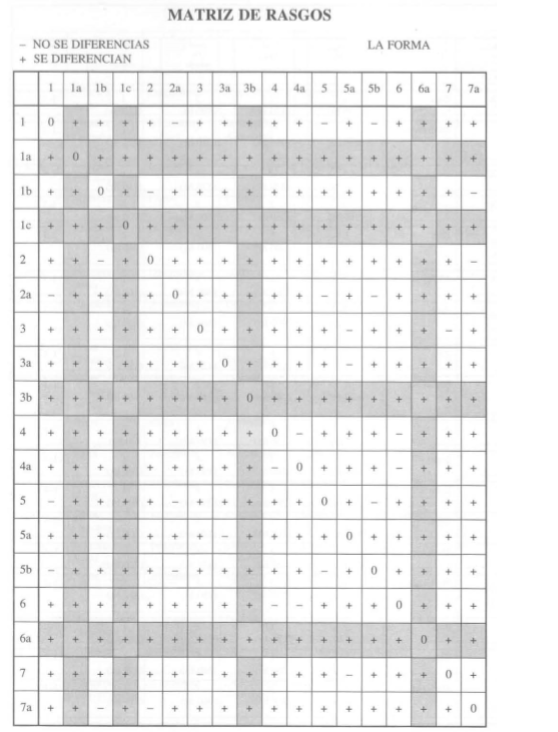
\includegraphics[width= 0.7\columnwidth]{Graphics/rasgos_forma}
\caption{Diferenciaci\'on en cuanto a la \emph{forma} de la curva mel\'odica. Tomado de \cite[p.220]{garcia1996aspectos2}.}
\label{rasgos_forma}
\end{center}
\end{figure}


\begin{figure}
\begin{center}
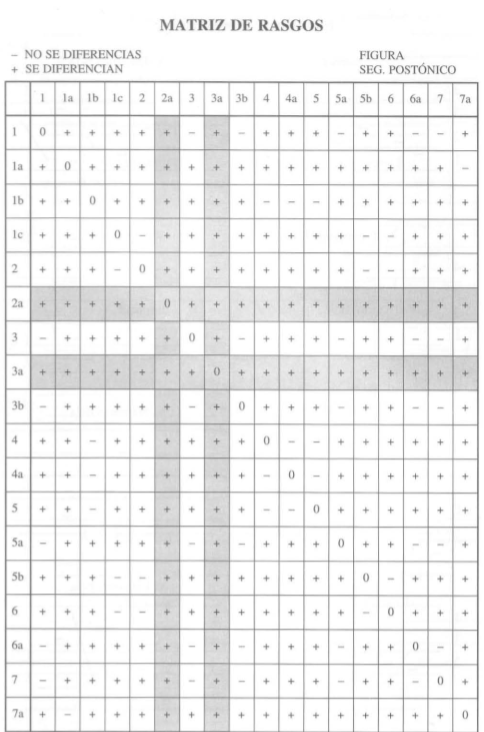
\includegraphics[width= 0.7\columnwidth]{Graphics/rasgos_figura}
\caption{Diferenciaci\'on en cuanto a la \emph{figura del segmento post\'onico}. Tomado de \cite[p.221]{garcia1996aspectos2}.}
\label{rasgos_figura}
\end{center}
\end{figure}


\begin{figure}
\begin{center}
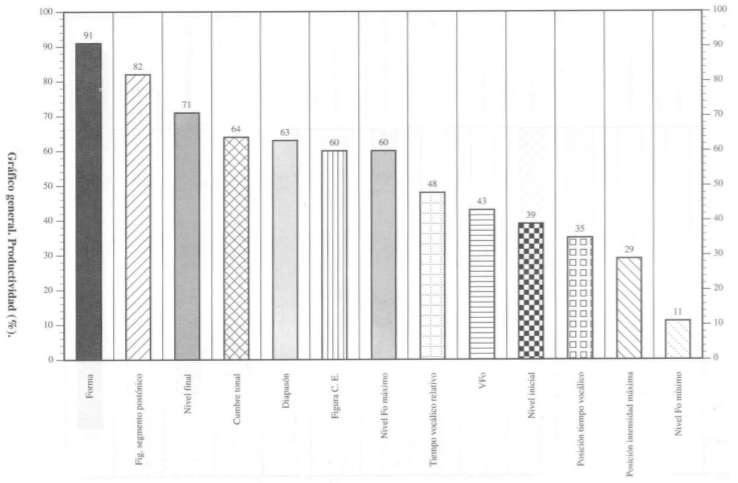
\includegraphics[width= 0.7\columnwidth]{Graphics/productividad}
\caption{Productividad de los rasgos distintivos en la investigaci\'on de Garc\'ia River\'on. Tomado de \cite[p.233]{garcia1996aspectos2}.}
\label{productividad}
\end{center}
\end{figure}

\begin{figure}
\begin{center}
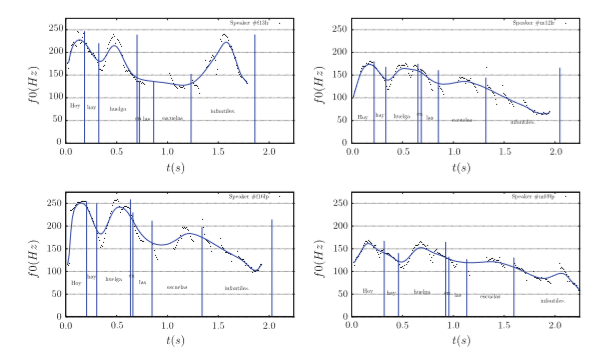
\includegraphics[width= 1\columnwidth]{Graphics/diferencialocutor}
\caption{Contorno mel\'odico de la frase ``Hoy hay huelga en las escuelas infantiles'' pronunciado por 4 individuos diferentes. Tomado de \cite[p.966]{garrido2013glissando}.}
\label{diferencialocutor}
\end{center}
\end{figure}


\begin{figure}
\begin{center}
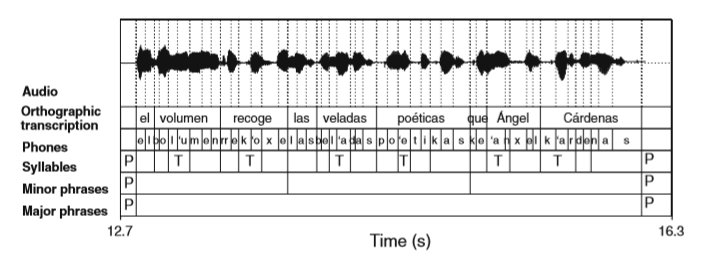
\includegraphics[width= 1\columnwidth]{Graphics/textgrid}
\caption{TextGrid de Praat de ejemplo. Tomado de \cite[p.962]{garrido2013glissando}.}
\label{textgrid}
\end{center}
\end{figure}


\begin{figure}
\begin{center}
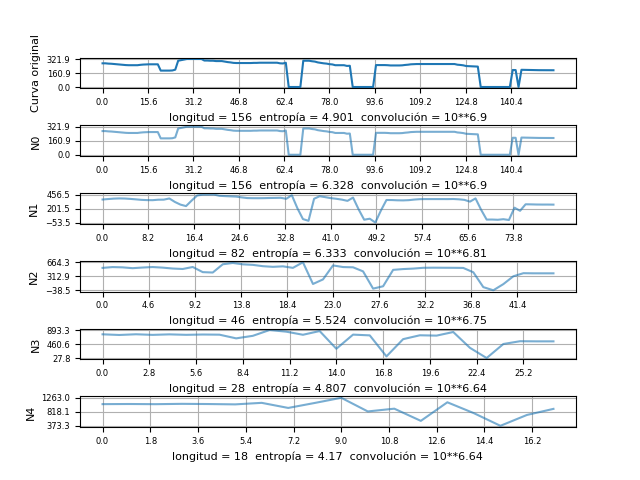
\includegraphics[width= 1\columnwidth]{Graphics/reconstruccion}
\caption{Reconstrucci\'on de la curva mel\'odica con los coeficientes de aproximaci\'on y de detalle de los niveles 0 al 4 en la DWT con Daubechies. Se muestra la entrop\'ia de la curva reconstruida en cada nivel, la longitud de la misma y su convoluci\'on con la curva original.}
\label{reconstruccion}
\end{center}
\end{figure}


\begin{figure}
\begin{center}
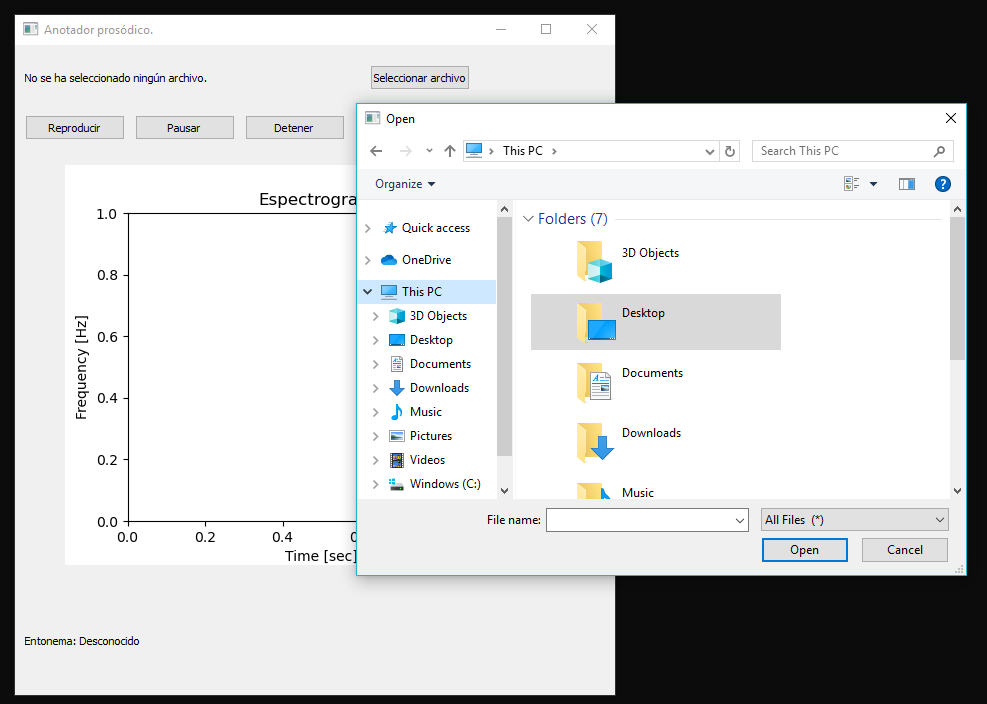
\includegraphics[width= 1\columnwidth]{Graphics/software}
\caption{Interfaz gr\'afica del software desarrollado. Su uso es simple: al presionar el bot\'on \emph{Seleccionar archivo} aparece un cuadro de di\'alogo para explorar y seleccionar el .wav que se desea analizar. Autom\'aticamente se grafica el espectrograma asociado y se muestra en la etiqueta inferior izquierda el entonema que se predice para el archivo seleccionado. Los botones \emph{Reproducir}, \emph{Pausar} y \emph{Detener} son para manipular el audio que est\'e seleccionado, cuyo nombre se muestra en la etiqueta superior izquierda. Un resultado de ejemplo se observa en la Figura \ref{software2}.}
\label{software}
\end{center}
\end{figure}

\begin{figure}
\begin{center}
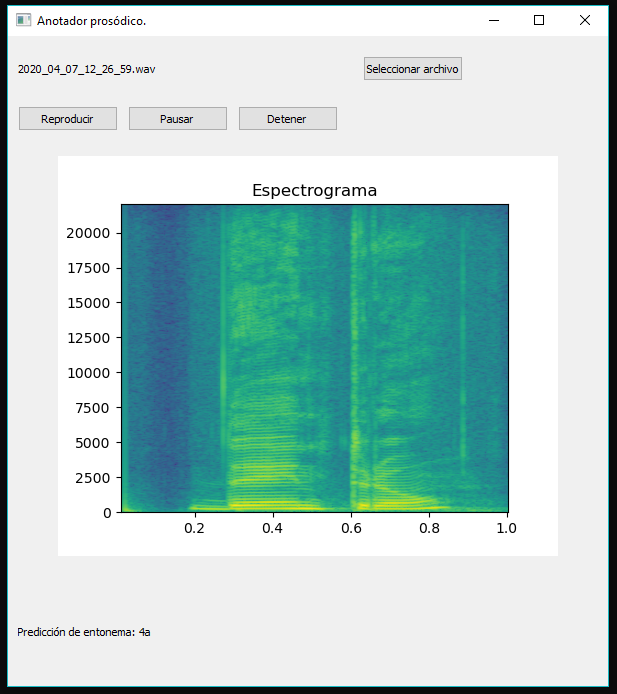
\includegraphics[width= 1\columnwidth]{Graphics/software2}
\caption{Interfaz gr\'afica del software desarrollado. Se muestra el espectrograma para el audio 2020\_04\_07\_12\_26\_59.wav y se predice por el algoritmo de aprendizaje que presenta el entonema \emph{4a}.}
\label{software2}
\end{center}
\end{figure}
%\bibliographystyle{plane}
%\bibliographystyle{dinat}
\bibliographystyle{unsrt} 


%\bibliographystyle{babplain-uh}
\bibliography{Bibliography}


\end{document}